\section{Обрада података, модели и дестилација}

У овом поглављу су описани скупови података који се користе у експериментима, као и модели машинског учења који служе као учитељи у процесу дестилације. Након тога је представљен процес дестилације помоћу ИЛП система \textit{Aleph}, укључујући конфигурацију и параметре који су коришћени.

\subsection{Скупови података}

У експериментима су коришћена два класична скупа података из \emph{UCI} репозиторијума преко \emph{OpenML}-а, а то су \emph{Mushroom} и \emph{Adult}. Обрада и припрема података је обављена у \emph{Python}-у помоћу библиотека \emph{pandas} и \emph{scikit-learn}.

Изворни код и \emph{Docker} конфигурација јавно су доступни у репозиторијуму \url{https://github.com/ristic-ac/Matematika-DAS}.

\paragraph{Окружење.}
Експерименти су извођени у \emph{Docker} окружењу заснованом на \emph{python:3.12-slim-bookworm}. Коришћене компоненте:
\begin{itemize}
  \item \emph{Python} 3.12,
  \item \emph{scikit-learn} уз \emph{XGBoost},
  \item \emph{SWI-Prolog},
  \item \emph{Aleph} пакет у \emph{SWI-Prolog}-у,
  \item \emph{Docker}.
\end{itemize}

\paragraph{Напомена о редоследу припреме података}
У спроведеним експериментима примењен је следећи редослед:
\begin{itemize}
  \item балансирање скупа одстрањивањем дела већинске класе,
  \item дискретизација (биновање) атрибута,
  \item обука модела и индукција правила.
\end{itemize}
У методолошкој литератури уобичајено је разматрати и алтернативне распореде корака (нпр.\ биновање пре балансирања) како би се умањио ризик од померања расподела и губитка унутар-класне варијабилности. Због временских и рачунарских ограничења, поновна обрада у алтернативном распореду није спроведена, те је задржан наведени поступак као прагматичан компромис.

\paragraph{Напомена} Све мере перформанси које ће бити приказане у наставку односе се на тест скуп који није коришћен ни у једном кораку обуке или оптимизације модела.
 
\subsubsection{\emph{Mushroom}}

\paragraph {О скупу података} \emph{Mushroom} је класичан скуп података са \emph{UCI} репозиторијума, доступан преко OpenML-а (верзија 1). Циљ је бинарна класификација јестиво/отровно. Сви атрибути су категорички (облик и боја шешира, лиске, стабљика, прстен, мирис и сл.), што га чини погодним за алгоритме који добро раде са номиналним карактеристикама. Позитивна класа је \textit{poisonous} (отровно).


\paragraph{Узорци} Скуп садржи укуп 8124 примера, од чега је 4208 јестиво, а 3916 отровно. Сваки пример има 22 атрибута (укључујући циљну променљиву).

\paragraph{Недостајуће вредности} Испоставља се да скуп садржи недостајуће вредности у атрибуту \textit{stalk-root} (стабљика). Недостајуће вредности су накнадно означене са \texttt{Unknown}.

\paragraph{Балансирање класа} Пре обуке је обезбеђен баланс између класа коришћењем \textit{undersampling} технике, тако да је број примера у обе класе једнак (3916). Коришћена је техника насумичног одбацивања примера из већинске класе.

\subsubsection{\emph{Adult}}

\paragraph{О скупу података} \emph{Adult} (верзија 2) је широко коришћен скуп за предвиђање прихода (>50K насупрот <=50K). Садржи мешавину нумеричких (нпр. \textit{age}, \textit{hours-per-week}, \textit{capital-gain}/\textit{capital-loss}) и категоричких (нпр. \textit{workclass}, \textit{education}, \textit{occupation}, \textit{native-country}) променљивих. Позитивна класа је \textit{>50K}.

\paragraph{Узорци} Скуп садржи 48842 примера, од чега је 11687 у класи >50K. Сваки пример има 15 атрибута (укључујући циљну променљиву).

\paragraph{Дискретизација нумеричких атрибута} Нумерички атрибути су дискритизовани у категорије: старост у старосне групе (нпр. <25, 25–35, итд.), сати рада недељно у интервале (нпр. ≤20, 21–40, итд.), капитални приходи и губици у категорије (0, \textit{small}, \textit{medium}, \textit{high}) према квартилним праговима, тежински фактор лог-трансформисан и подељен на квартиле, а образовање груписано у \textit{Below\_HS}, \textit{HS\_Graduate}, \textit{Some\_College}, \textit{Bachelors}, \textit{Advanced\_Degree} и \textit{Other}.

\paragraph{Балансирање класа} Како би се смањила неуравнотеженост између класа, примењена је \textit{undersampling} техника на већинску класу (<=50K), тако да је број примера у обе класе једнак (11687). Ово је постигнуто насумичним одбацивањем примера из већинске класе.

\subsection{Модели машинског учења}
\paragraph{Примена модела} У овом делу рада примењени су класични алгоритми машинског учења над обрађеним скуповима података. Као базни модели изабрани су стабло одлуке (\emph{Decision Tree}, \textit{DT}), случајне шуме (\emph{Random Forest}, \textit{RF}) и \emph{XGBoost} (\textit{XGB}). Ови алгоритми представљају добру комбинацију једноставних и напредних техника заснованих на стаблима, што омогућава поређење перформанси у односу на сложеност модела.

\paragraph{Подела скупа и оптимизација} За све моделе примењена је подела скупа на део за тренирање (85\%) и тестирање (15\%), уз стратификовано узорковање како би се очувала расподела класа. Избор најбољих хиперпараметара извршен је коришћењем \textit{Grid Search}-а са унакрсном валидацијом (\textit{5-fold cross-validation}), при чему је критеријум оптимизације била тачност (\textit{accuracy}).

\paragraph{Анализа значајности особина} Код модела који подржавају израчунавање значајности особина (\textit{DT}, \textit{RF}, \textit{XGB}), спроведена је анализа feature importances. Ово не само да омогућава боље разумевање релевантности појединачних атрибута у процесу класификације, већ и смањује сложеност даље обраде у систему Aleph, пошто се небитне особине искључују из простора претраге правила. Одабрана су најзначајнија обележја која покривају преко 90\% укупне важности.

\subsubsection{Mushroom}

\paragraph{Decision Tree (DT)}
Accuracy: \textbf{99.06\%}\\
Најзначајније особине: \textit{spore-print-color}, \textit{ring-number}, \textit{gill-size}.\\
Оптимални хиперпараметри: \texttt{criterion=gini}, \texttt{max\_depth=8}, \texttt{min\_samples\_leaf=1}.\\
Напомена: модел остаје компактан, без уочљивог преобучавања.

\paragraph{Random Forest (RF)}
Accuracy: \textbf{100.00\%}\\
Најзначајније особине: \textit{spore-print-color}, \textit{odor}, \textit{gill-size}, \textit{ring-type}.\\
Оптимални хиперпараметри: \texttt{criterion=gini}, \texttt{max\_depth=None}, \texttt{min\_samples\_leaf=1}, \texttt{n\_estimators=50}.\\
Напомена: ансамблирање стабала у потпуности елиминише грешке и стабилизује процене значајности.

\paragraph{XGBoost}
Accuracy: \textbf{99.23\%}\\
Најзначајније особине: \textit{spore-print-color}, \textit{ring-number}, \textit{gill-size}, \textit{veil-color}, \textit{gill-spacing}, \textit{ring-type}, \textit{odor}.\\
Оптимални хиперпараметри: \texttt{learning\_rate=0.01}, \texttt{max\_depth=5}, \texttt{n\_estimators=200}, \texttt{subsample=0.8}.\\
Напомена: додатна сложеност не доноси добит на високо раздвојивом скупу.

\medskip
\noindent\textit{Поређење (Mushroom):} \textit{RF} = 100\% $>$ \textit{XGBoost} (99.23\%) $>$ \textit{DT} (99.06\%).

\subsubsection{Adult}

\paragraph{Decision Tree (DT)}
Accuracy: \textbf{80.73\%}\\
Најзначајније особине: \textit{relationship}, \textit{education}, \textit{capital-gain}, \textit{age}.\\
Оптимални хиперпараметри: \texttt{criterion=gini}, \texttt{max\_depth=10}, \texttt{min\_samples\_leaf=10}.\\
Напомена: снажан базни резултат, осетљивији на варијансу од ансамбл приступа.

\paragraph{Random Forest (RF)}
Accuracy: \textbf{81.53\%}\\
Најзначајније особине: \textit{relationship}, \textit{marital-status}, \textit{education}, \textit{age}, \textit{capital-gain}, \textit{occupation}, \textit{hours-per-week}, \textit{sex}.\\
Оптимални хиперпараметри: \texttt{criterion=gini}, \texttt{max\_depth=20}, \texttt{min\_samples\_leaf=5}, \texttt{n\_estimators=100}.\\
Напомена: стабилнији и благо бољи резултати у односу на \textit{DT} услед смањења варијансе.

\paragraph{XGBoost}
Accuracy: \textbf{82.28\%}\\
Најзначајније особине: \textit{relationship}, \textit{education}, \textit{marital-status}, \textit{capital-gain}, \textit{age}, \textit{hours-per-week}, \textit{capital-loss}, \textit{occupation}.\\
Оптимални хиперпараметри: \texttt{learning\_rate=0.2}, \texttt{max\_depth=3}, \texttt{n\_estimators=100}, \texttt{subsample=1.0}.\\
Напомена: најбољи скор међу тестираним моделима на овом скупу.

\medskip
\noindent\textit{Поређење (Adult):} \textit{XGBoost} (82.28\%) $>$ \textit{RF} (81.53\%) $>$ \textit{DT} (80.73\%).


\subsection{Дестилација модела}

У овом делу рада примењена је дестилација модела машинског учења у облик логичких правила коришћењем ИЛП система \emph{Aleph}. Овај процес укључује неколико корака, укључујући припрему података, конфигурацију Aleph-а и анализу добијених правила.

\paragraph{Припрема података} За сваки скуп података (\emph{Mushroom} и \emph{Adult}) припремљени су Prolog фајлови који садрже позитивне и негативне примере на основу предвиђања изабраних модела машинског учења (\textit{DT}, \textit{RF}, \textit{XGB}). Поред тога, дефинисан је скуп позадинског знања који укључује релевантне особине из сваког скупа.

\paragraph{Конфигурација \emph{Aleph}-а} \emph{Aleph} је конфигурисан са различитим поставкама како би се истражио утицај на сложеност и перформансе добијених правила. Три различите поставке су коришћене: \textit{sniper}, \textit{sweet\_spot} и \textit{sweeper}, које варирају у параметрима као што су стратегија претраге, ограничење броја чворова, функција евалуације и минимална подршка.

\paragraph{Интуитивни мотив и очекивани профил пресета}
Поставке су конципиране тако да покрију три режима понашања система. \textit{sniper} тежи максимизацији прецизности: користе се строжи критеријуми прихватања, ограниченија претрага (нижи лимит чворова) и евалуација која фаворизује тачност и нижим покрићем. \textit{sweeper} ради супротно: проширује простор претраге (виши лимити, шира стратегија), ублажава праг прихватања и тежи већем покрићем, уз умерену прецизност. \textit{sweet\_spot} поставка поставља параметре између ове две крајности са циљем да се постигне уравнотежен компромис између прецизности, покрића и сложености модела. Апсолутне вредности (број правила и просечна дужина тела) зависе од скупа података и претпроцесирања, извештавају се у резултатима као оријентир за избор пресета: \emph{sniper} за високу поузданост локалних објашњења, \emph{sweeper} за дескриптивну експлорацију простора, а \emph{sweet\_spot} као подразумевана опција за интерпретабилност уз рачунску ефикасност.

\paragraph{Параметри Aleph-а} Кључни параметри који су коришћени у Aleph-у су следећи:

\begin{itemize}
    \item \texttt{search} - стратегија претраге клауза:
    \begin{itemize}
        \item \texttt{heuristic} - најбоље-прво (best-first) по корисности;
        \item \texttt{bf} - претрага по ширини (краће клаузе пре дужих, затим по корисности).
    \end{itemize}
    \item \texttt{openlist} - „ширина снопа“ (beam width): горња граница броја кандидата у листи отворених клауза које се даље разматрају.
    \item \texttt{nodes} - максималан број обрађених чворова/кандидат-клауза у једној потрази за клаузом.
    \item \texttt{evalfn} — функција вредновања кандидата:
    \begin{itemize}
        \item \texttt{laplace} — глатка прецизност \((P+1)/(P+N+2)\);
        \item \texttt{wracc} — тежинска релативна тачност (компромис између тачности и покривености);
        \item \texttt{coverage} — покривеност са казном за негативне \((P-N)\).
    \end{itemize}
    \item \texttt{clauselength} — максимална дужина тела клаузе (број литерала), тј. ограничење сложености правила.
    \item \texttt{minacc} — минимална „тачност“ клаузе (у Aleph-у то је прецизност \(\frac{P}{P+N}\)); клаузе испод овог прага се одбацују.
    \item \texttt{minpos} — минималан број позитивних примера које клауза мора да покрије (штити од превише уских правила).
    \item \texttt{noise} — максимално дозвољен број негативних примера које клауза сме да покрије (толеранција на шум/лажне позитиве). \cite{aleph_manual}
\end{itemize}

Главе правила су увек исте: \texttt{class(X, positive)}, у завиности од циљне класе. Тела клауза се састоје од литерала који представљају атрибуте и њихове вредности, па су тако у оквиру дестилације обележја чија укупна важност прелази 90\% (из претходне анализе) представљена као улазни литерали. Сваки литерал има детерминистичност 1, што значи да се увек појављује у телу клаузе највише једном.

У наредним поглављима анализира се квалитет дестилације модела кроз поређење перформанси дестилата у односу на две референтне: \emph{истину} (ground truth) и \emph{учитеља} (teacher). За сваку комбинацију модела и пресета (\textit{dt}, \textit{rf}, \textit{xgb} × \textit{sniper}, \textit{sweet\_spot}, \textit{sweeper}) процењује се пет стандардних метрика бинарне класификације: \textit{accuracy}, \textit{precision}, \textit{recall}, \textit{F1} и \textit{MCC}. Поред стандардних метрика, разматране су вредности броја правила и просечне дужине тела клауза као индикатори сложености модела.
Кључни аспект је разликовање \textbf{верности} (фиделитета, односно тачност према учитељу) учитељу од \textbf{стварне тачности} према истини (тачност према реалним ознакама). Дестилати могу веома добро имитирати учитеља (висок фиделитет), а да притом не побољшају реалан квалитет према истинитим ознакама.
Поређења су приказана засебно за \textit{mushroom} (лако раздвојив, често близу „максимума“) и \textit{adult} (умерено захтеван) скуп. 

\subsubsection{Mushroom}

У табели \ref{tab:aleph-mushroom} су приказана Aleph подешавања за скуп \textit{mushroom}, која су иста за све учитељске моделе (\textit{DT}, \textit{RF}, \textit{XGB}). 

\begin{table}[H]
\centering
\small
\setlength{\tabcolsep}{4pt}
\begin{tabularx}{\textwidth}{@{} l c c c c c c c c @{}}
\toprule
\textbf{Поставка} & \texttt{search} & \texttt{openlist} & \texttt{nodes} & \texttt{evalfn} & \texttt{cl} & \texttt{minacc} & \texttt{minpos} & \texttt{noise} \\
\midrule
sniper      & heuristic & 40   & 80k  & laplace  & 3 & 0.90 & 5 & 1  \\
sweet\_spot & heuristic & 64   & 100k  & wracc    & 3 & 0.80 & 5 & 5  \\
sweeper     & bf        & 1000 & 150k & coverage & 3 & 0.70 & 5 & 20 \\
\bottomrule
\caption{Aleph подешавања за \textit{mushroom}, иста за \textit{DT}/\textit{RF}/\textit{XGB}. Напомена: \texttt{cl} означава \texttt{clauselength}.}
\label{tab:aleph-mushroom}
\end{tabularx}
\end{table}

\paragraph{Резултати} Табела \ref{tab:ilp-mushroom} приказује перформансе дестилованих ИЛП модела у односу на сложеност, са метрикама као што су тачност (accuracy), \textit{MCC}, фиделитет, број правила и просечна дужина тела правила. На дијаграмима расејања су поједини записи означени својим \emph{ID}-јем, који се може наћи у табели.

Све конфигурације дају поприлично висок фиделитет, преко 95\%, чак и оне са малим бројем правила и једноставним телима клаузи. Парето фронт показује да се већ са врло једноставним моделима постиже максимум, па сложенији модели не доносе додатну вредност, видети слику \ref{fig:mush-complexity-fidelity}.
\begin{figure}[H]
  \centering
  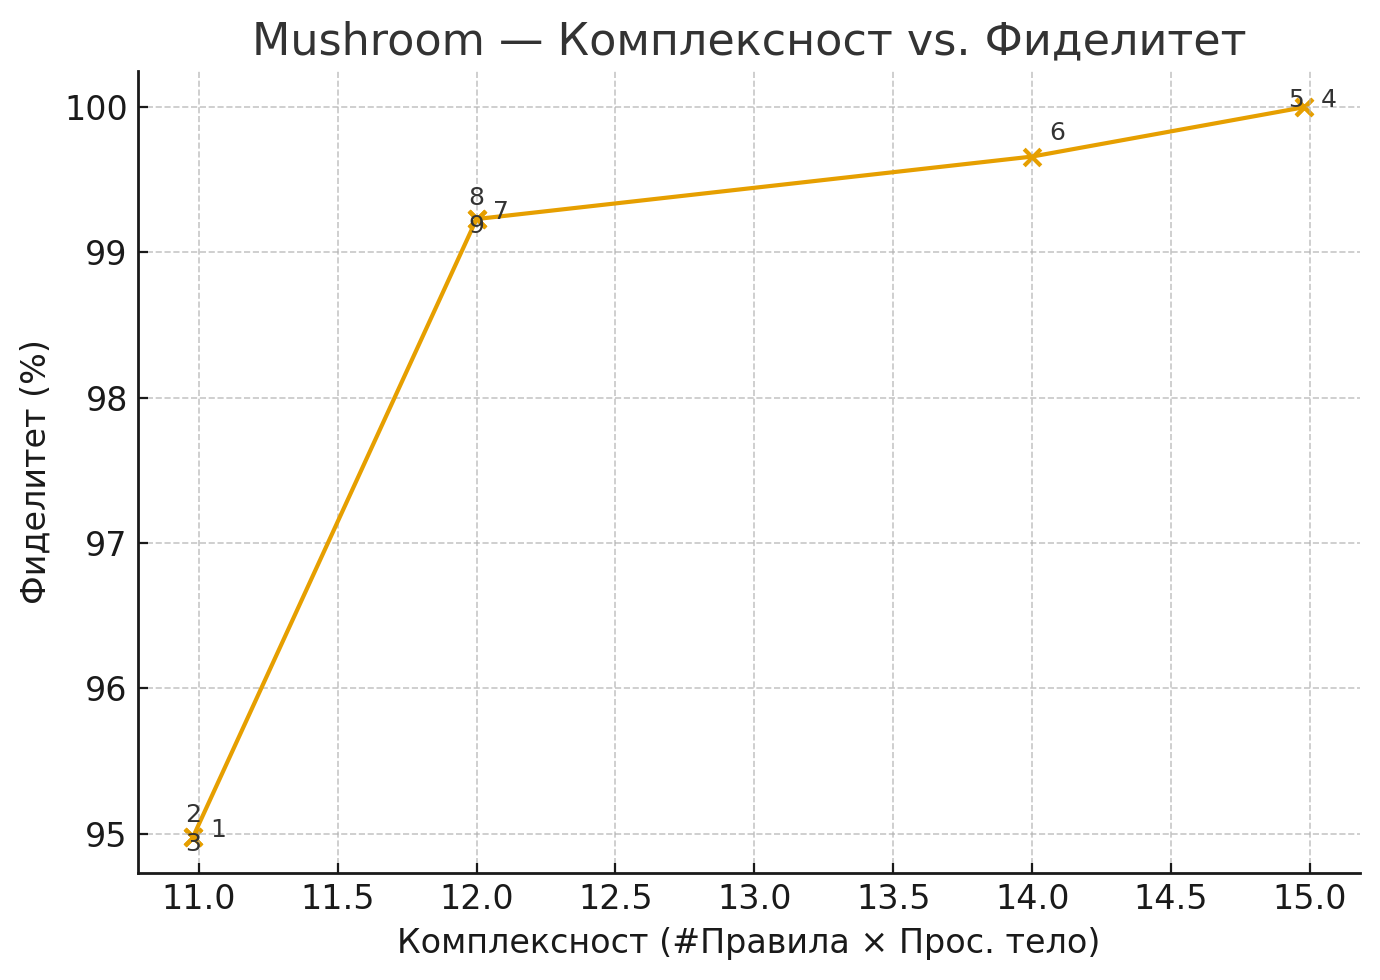
\includegraphics[width=.85\linewidth]{images/charts/mushroom-kompleksnost-fidelitet.png}
  \caption{Комплексност vs. Фиделитет — \textit{mushroom}.}
  \label{fig:mush-complexity-fidelity}
\end{figure}

Све тачке постижу веома високу тачност, преко 96\%. Ово додатно потврђује да је скуп \textit{mushroom} лако раздвојив, те да чак и једноставни модели могу постићи скоро савршене резултате. Као и код фиделитета, Парето фронт показује да се већ са врло једноставним моделима постиже максимум, па сложенији модели не доносе додатну вредност, видети слику \ref{fig:mush-complexity-accuracy}.
\begin{figure}[H]
  \centering
  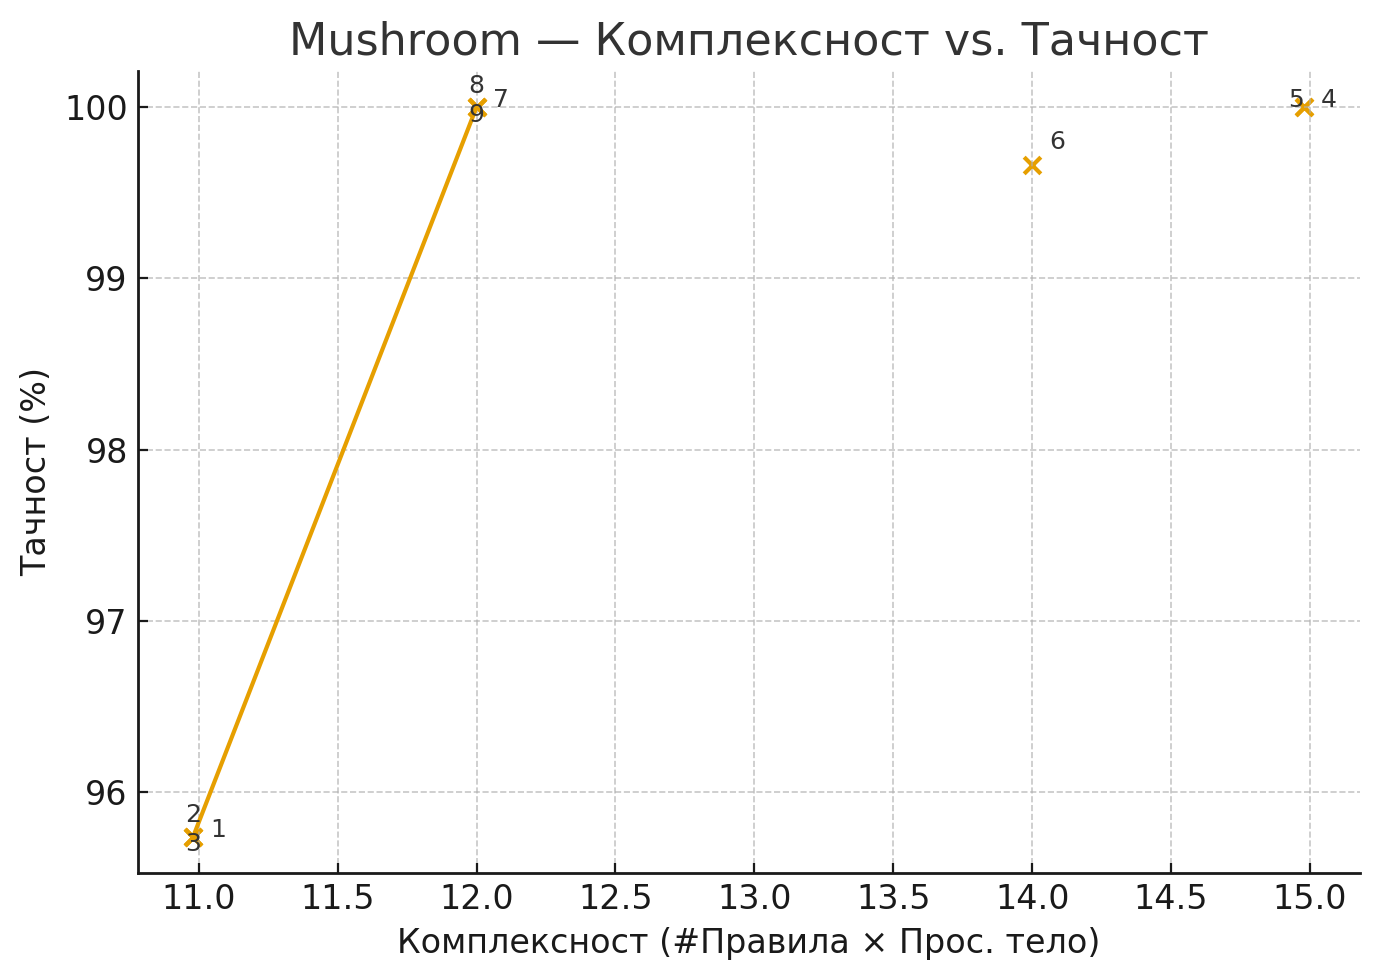
\includegraphics[width=.85\linewidth]{images/charts/mushroom-kompleksnost-tacnost.png}
  \caption{Комплексност vs. Тачност — \textit{mushroom}.}
  \label{fig:mush-complexity-accuracy}
\end{figure}

\textit{MCC} вредности су високе за све учитеље и све поставке, али \textit{DT} вредности су константно испод \textit{RF} и \textit{XGB}, што показује да ансамбл модели постижу бољу укупну корелацију предвиђања у односу на једноставније моделе, видети слику \ref{fig:mush-mcc}.
\begin{figure}[H]
  \centering
  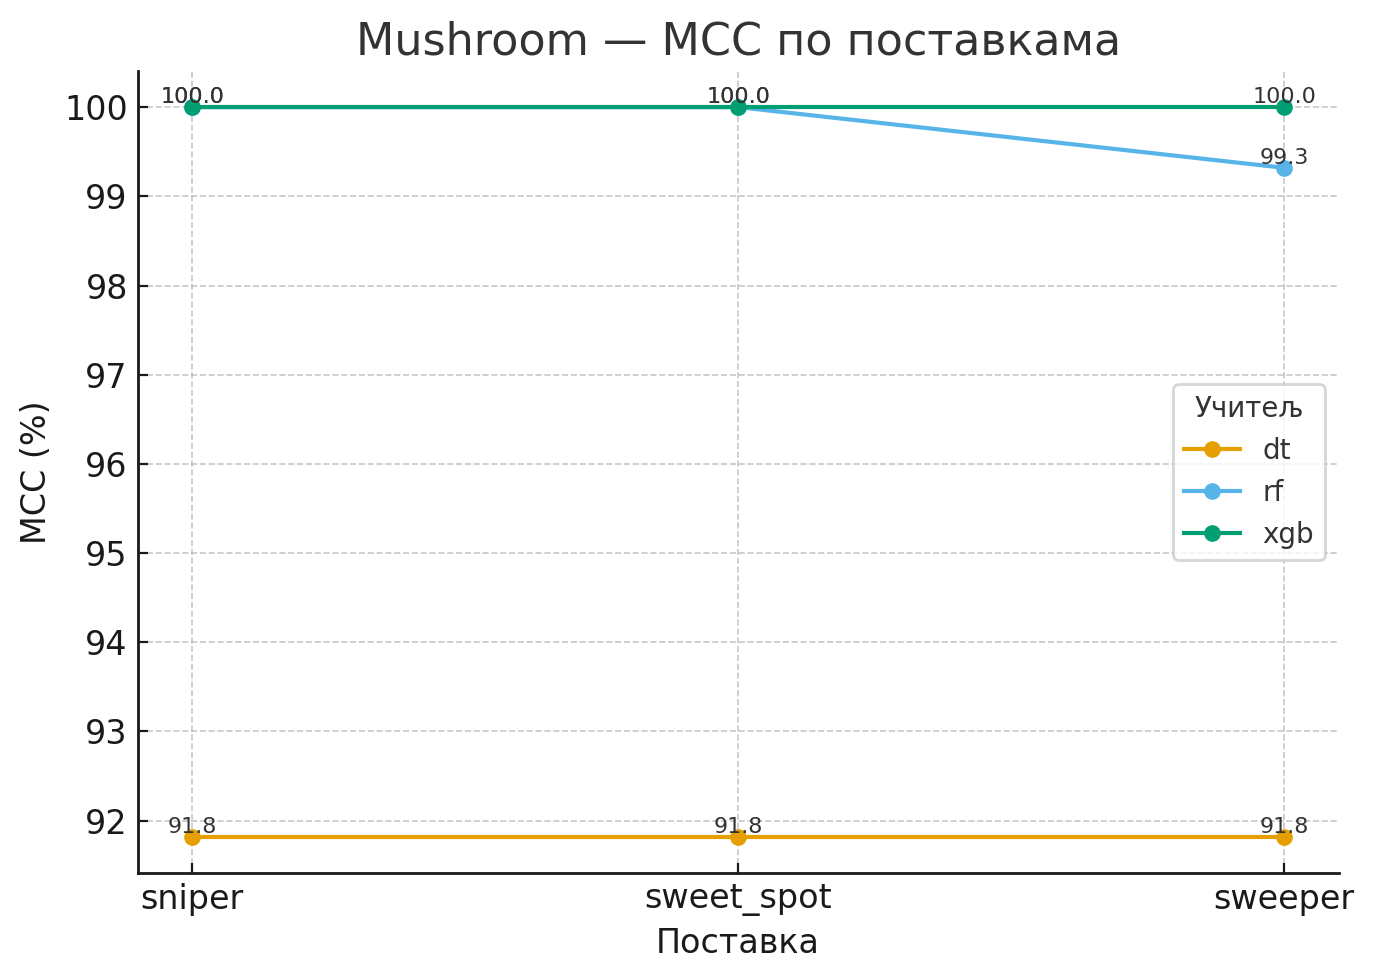
\includegraphics[width=.85\linewidth]{images/charts/mushroom-mcc.png}
  \caption{\textit{MCC} по поставкама — \textit{mushroom}.}
  \label{fig:mush-mcc}
\end{figure}

Табела \ref{tab:rules-top1-mushroom} приказује најбоље правило по комбинацији (датасет, учитељ, поставка). Правила су одабрана по највишој подршци.

\begin{table}[H]
\centering
\resizebox{\textwidth}{!}{
\begin{tabular}{@{}lllrrrrr@{}}
\toprule
\textbf{Скуп} & \textbf{Учитељ} & \textbf{Поставка} & \textbf{ИД правила} & \textbf{|Тело|} & \textbf{Подршка} & \textbf{Покривеност} & \textbf{Прецизност} \\
\midrule
mushroom & dt  & sniper     & 4  & 3 & 270 & 0.4530 & 1.0000 \\
mushroom & dt  & sweet\_spot& 4  & 3 & 270 & 0.4530 & 1.0000 \\
mushroom & dt  & sweeper    & 4  & 3 & 270 & 0.4530 & 1.0000 \\
mushroom & rf  & sniper     & 7  & 3 & 352 & 0.5997 & 1.0000 \\
mushroom & rf  & sweet\_spot& 7  & 3 & 352 & 0.5997 & 1.0000 \\
mushroom & rf  & sweeper    & 8  & 2 & 352 & 0.5997 & 1.0000 \\
mushroom & xgb & sniper     & 8  & 1 & 332 & 0.5589 & 1.0000 \\
mushroom & xgb & sweet\_spot& 8  & 1 & 332 & 0.5589 & 1.0000 \\
mushroom & xgb & sweeper    & 8  & 1 & 332 & 0.5589 & 1.0000 \\
\bottomrule
\end{tabular}
}
\caption{Најбоље правило за скуп \textit{mushroom} по комбинацији (учитељ, поставка), бирано по највишој подршци.}
\label{tab:rules-top1-mushroom}
\end{table}

Уочава се висока стабилност и понављање истих клауза кроз различите поставке и учитеље. Код \textit{DT} учитеља идентична тролитерална клауза $spore\_print\_color = white \land ring\_number = one \land gill\_spacing = close$ доследно се јавља у \textit{sniper}, \textit{sweet\_spot} и \textit{sweeper} поставкама са истом подршком (270) и прецизношћу (1.00). Код \textit{XGB} учитеља једнолитерална клауза $odor = foul$ понавља се у све три поставке (подршка 332, прецизност 1.00). Код \textit{RF} учитеља тролитерална клауза се јавља у \textit{sniper} и \textit{sweet\_spot}, док се у \textit{sweeper} поставци појављује њена редукована дволитерална верзија са истом подршком (352) и прецизношћу (1.00).

Ови налази указују на постојање врло чистих сепаратора класа, чија се структура мало мења са променом поставке. Разлике међу учитељима огледају се у избору атрибута: \textit{DT} фаворизује $spore\_print$ карактеристике, \textit{RF} физичке особине (нпр. модрице, површина), док \textit{XGB} даје приоритет мирису.

\paragraph{Напомена о наредним графиконима} У наредним графиконима, за сваку метрику, приказане су вредности у односу на учитеља и истину по свим комбинацијама учитељ/поставка. За сваку метрику приказан је засебан графикон.

Тачност према истини је једнака или незнатно виша од тачности према учитељу, многе комбинације су практично савршене. Ово указује да дестилат постиже бар онолико исправних предвиђања према истини колико и усклађених предвиђања са учитељем. Видети слику \ref{fig:mush-acc}.
\begin{figure}[H]
  \centering
  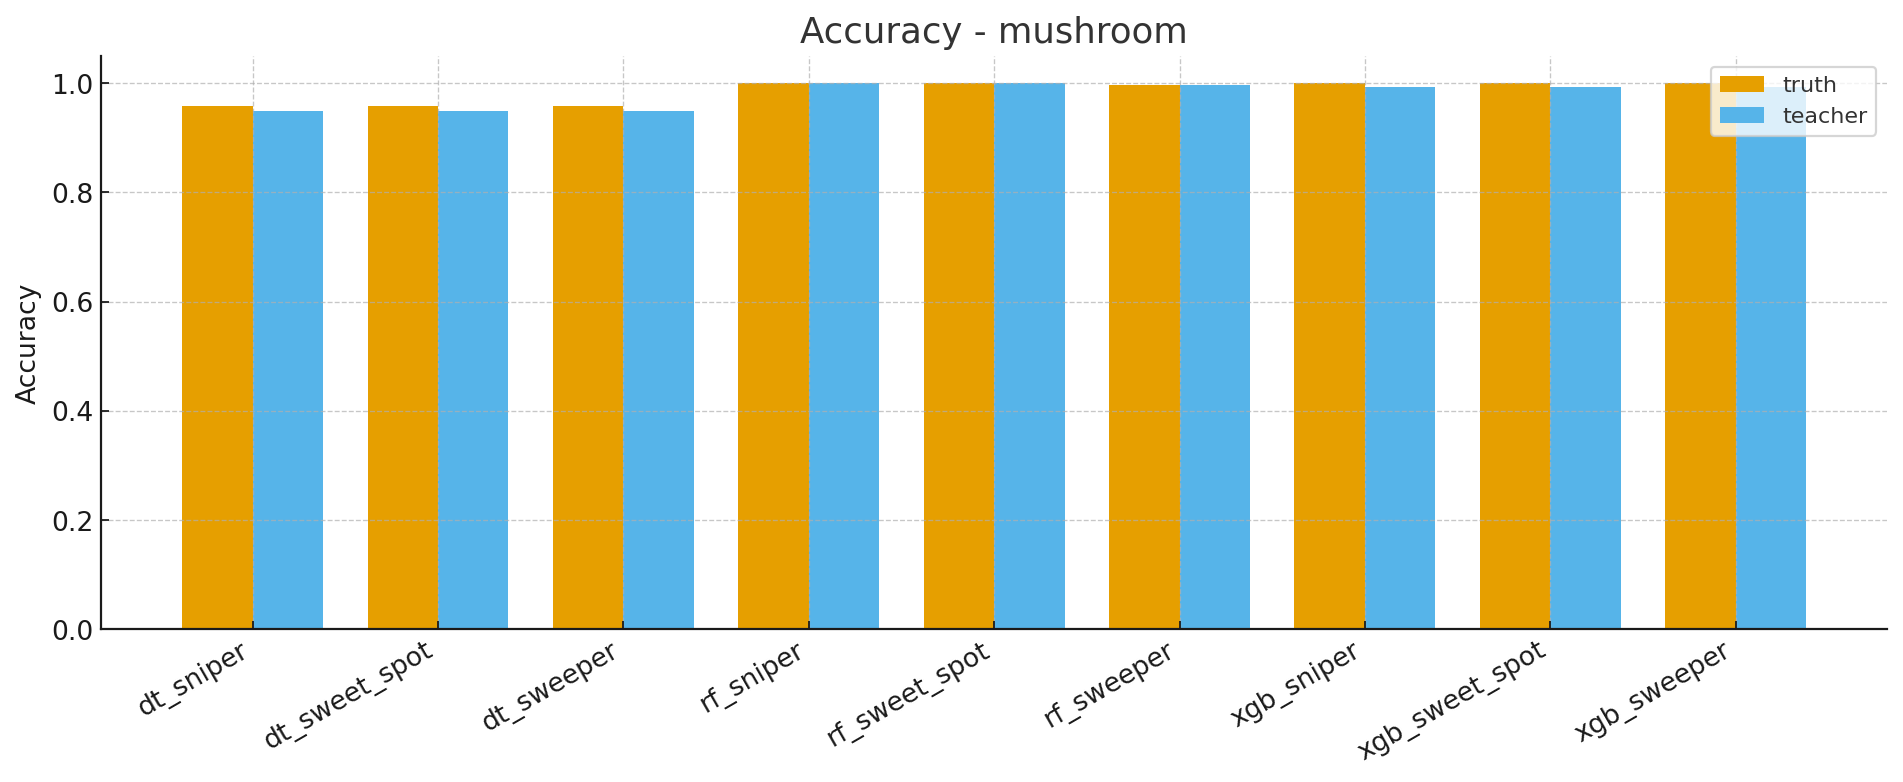
\includegraphics[width=.85\linewidth]{images/charts/accuracy_simple_mushroom.png}
  \caption{Accuracy — \textit{mushroom}.}
  \label{fig:mush-acc}
\end{figure}

Скоро све вредности су 1.0 (или врло близу) и према истини и према учитељу, позитивне прогнозе су истовремено коректне и усклађене са учитељем, уз минималне разлике. Видети слику \ref{fig:mush-prec}.
\begin{figure}[H]
  \centering
  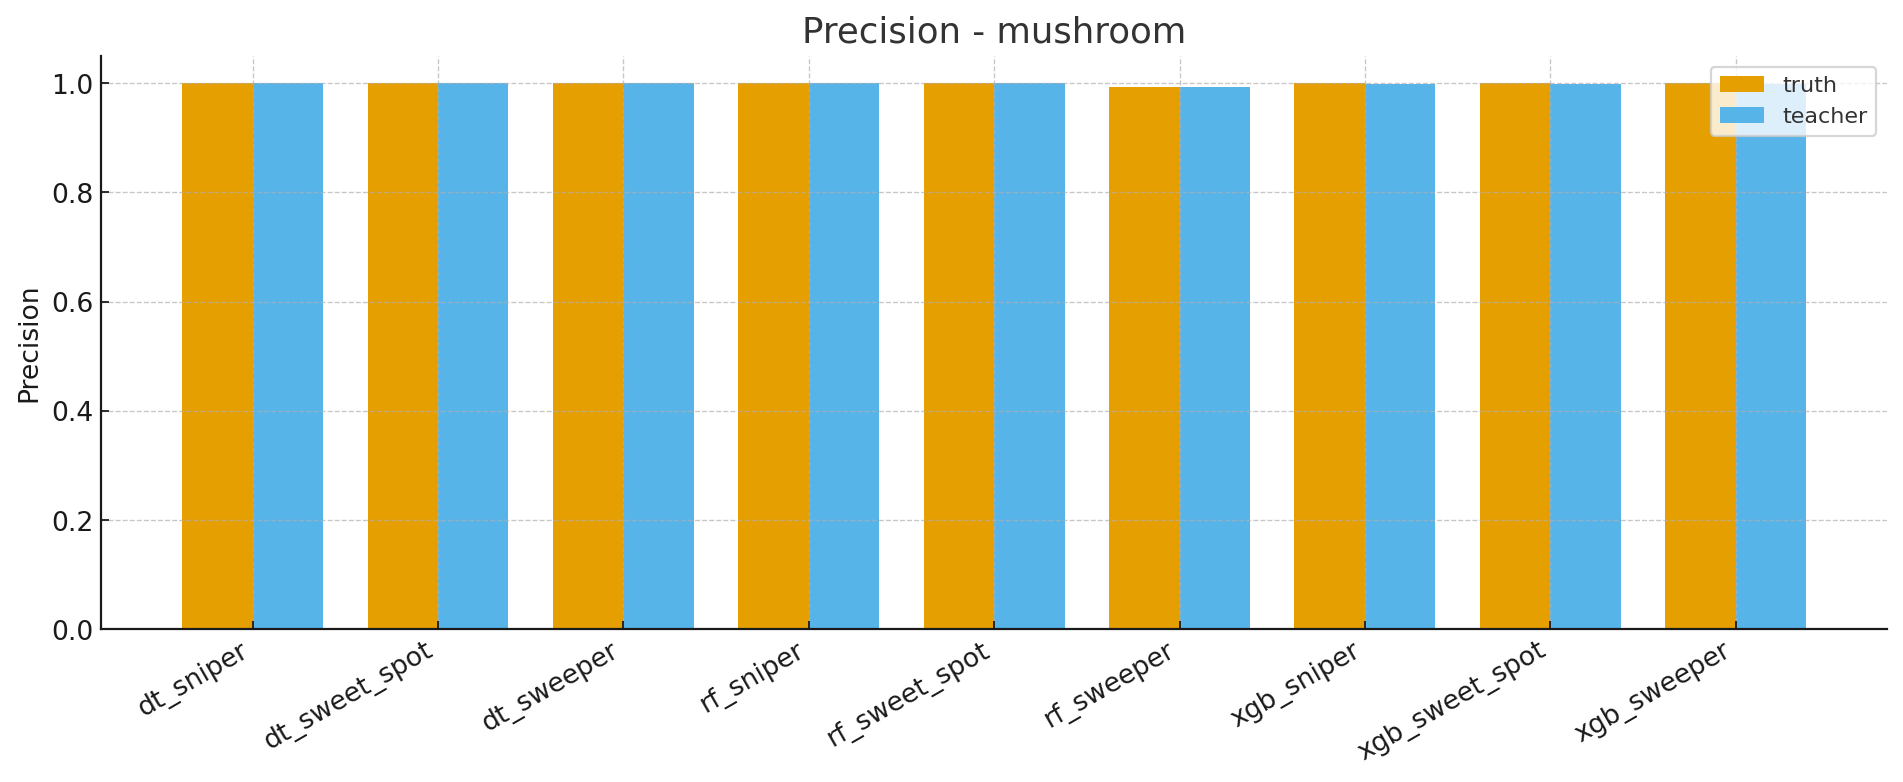
\includegraphics[width=.85\linewidth]{images/charts/precision_simple_mushroom.png}
  \caption{Precision — \textit{mushroom}.}
  \label{fig:mush-prec}
\end{figure}

Одзив према истини је једнак или нешто већи од одзива према учитељу (а за \texttt{rf} практично савршен у оба режима), што показује да дестилат идентификује готово све стварне позитиве и да га учитељев скуп позитивних примера не „ограничава“. Видети слику \ref{fig:mush-recall}.
\begin{figure}[H]
  \centering
  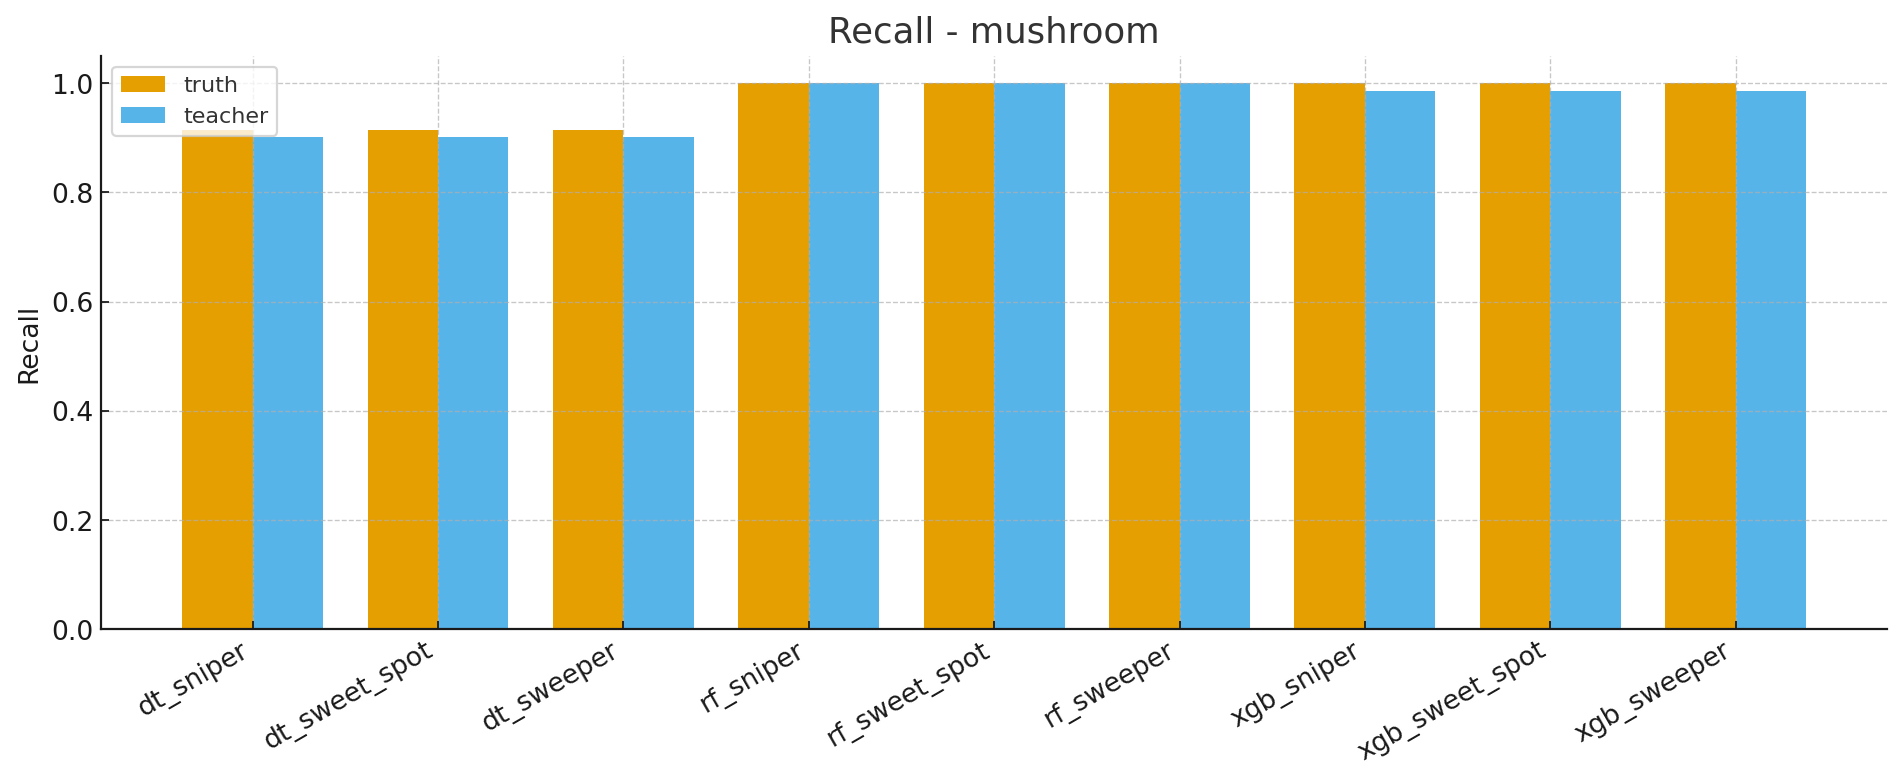
\includegraphics[width=.85\linewidth]{images/charts/recall_simple_mushroom.png}
  \caption{Recall — \textit{mushroom}.}
  \label{fig:mush-recall}
\end{figure}

F1 према истини је једнак или незнатно виши од F1 према учитељу (за \texttt{rf} савршен у оба), што значи да је стварни баланс прецизности и одзива најмање онолико добар колико и верност учитељу, још један показатељ перформанси које су близу максимума. Видети слику \ref{fig:mush-f1}.
\begin{figure}[H]
  \centering
  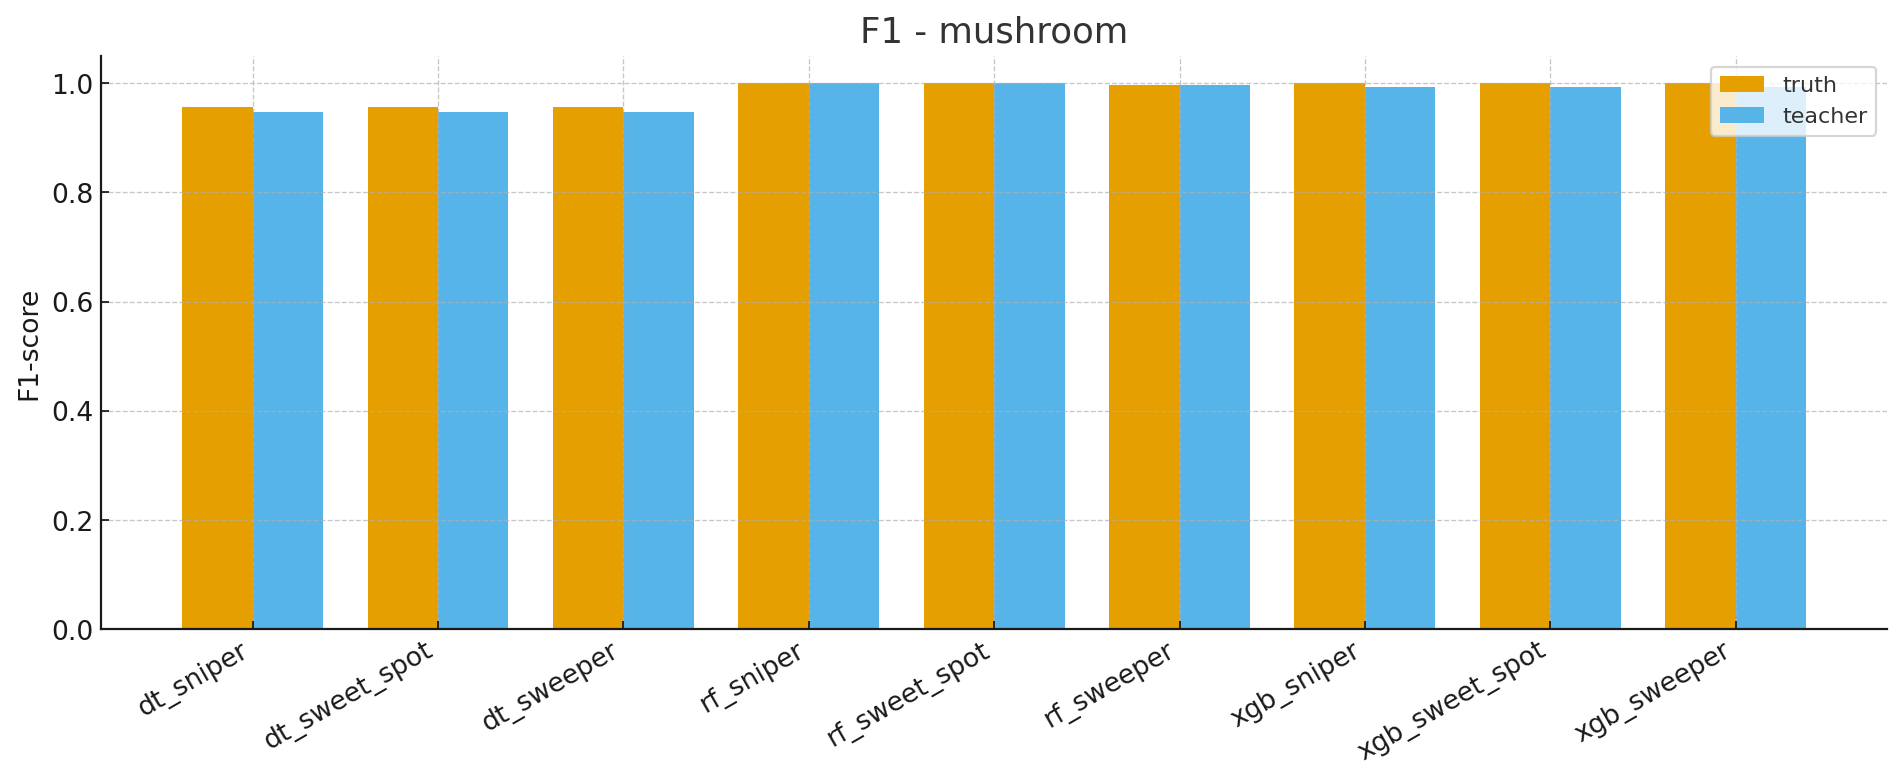
\includegraphics[width=.85\linewidth]{images/charts/f1_simple_mushroom.png}
  \caption{F1 — \textit{mushroom}.}
  \label{fig:mush-f1}
\end{figure}

\textit{MCC} према истини је једнак или нешто виши од \textit{MCC} према учитељу (за \texttt{rf} ≈ 1.0 у оба), што говори да је глобална усаглашеност са истинитим ознакама барем толико добра као и са учитељем, практично максимум перформанси на овом скупу. Видети слику \ref{fig:mush-mcc-tt}.
\begin{figure}[H]
  \centering
  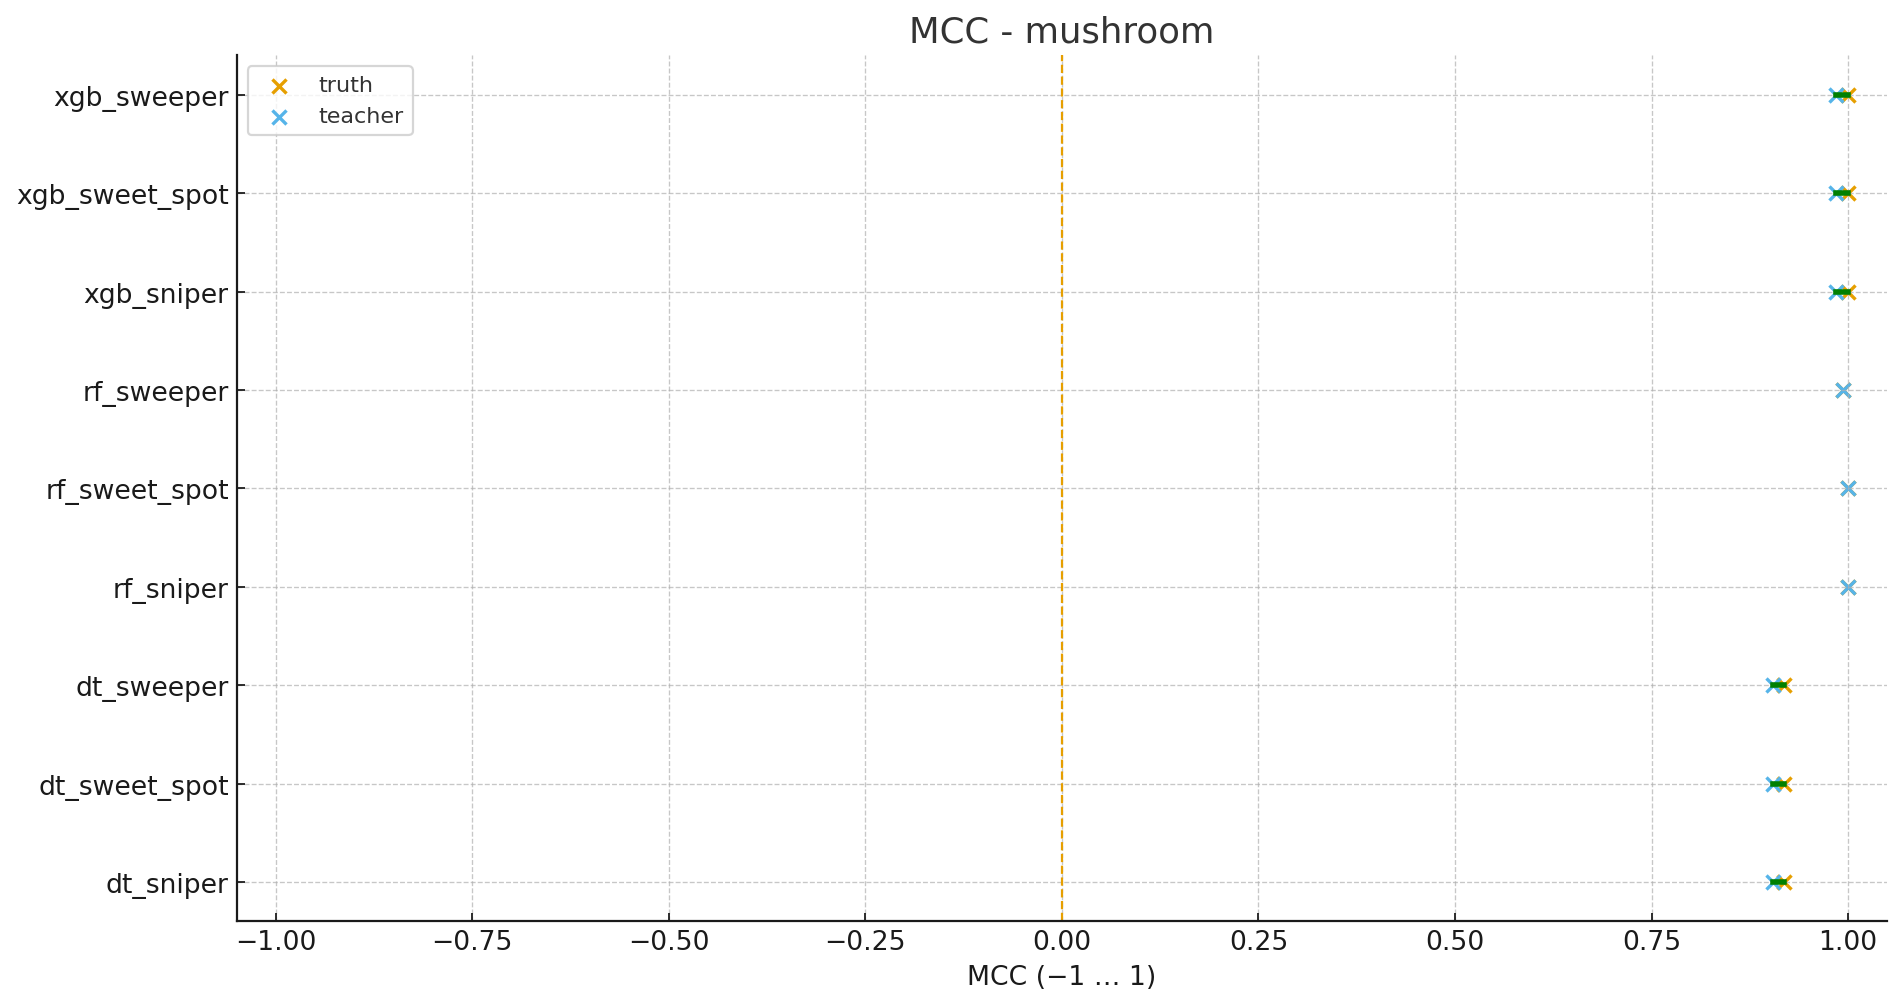
\includegraphics[width=.85\linewidth]{images/charts/mcc_simple_mushroom.png}
  \caption{\textit{MCC} — \textit{mushroom}.}
  \label{fig:mush-mcc-tt}
\end{figure}

\subsubsection*{Закључак — \textit{mushroom}}
На скупу \textit{mushroom} дестилација у Aleph-у даје готово савршене моделе: фиделитет је стабилно ≥95\%, а тачност ≥96\% у свим пресетима и за све учитеље. Парето анализа показује „колено“ већ при малом броју правила и кратким телима клауза, а додатна сложеност не доноси добит. \textit{MCC} је висок за све, при чему \textit{RF}/\textit{XGB} благо надмашују \textit{DT}. Најбоља правила су изузетно стабилна преко пресета (нпр. једнолитерално \texttt{odor=foul} код \textit{XGB}, \textit{spore print} карактеристике код \textit{DT}, физичке особине код \textit{RF}), што потврђује постојање „чистих“ сепаратора класа. Перформансе према истини су једнаке или незнатно више од перформанси према учитељу, па је дестилат и веродостојан и коректан. Практично, препоручљиве су једноставније поставке (\texttt{heuristic} претрага, мањи \texttt{clauselength}, конзервативан \texttt{minacc}, низак \texttt{noise}). Овај скуп је, дакле, лако раздвојив и омогућава максималну објашњивост без губитка квалитета.


%%% ADULT %%%
\subsubsection{Adult}

У табели \ref{tab:aleph-adult} су приказана Aleph подешавања за скуп \textit{adult}, која варирају у зависности од учитељског модела и поставке.

\begin{table}[H]
\centering
\small
\setlength{\tabcolsep}{3pt}
\begin{tabularx}{\textwidth}{@{} l l c c c c c c c c @{}}
\toprule
\textbf{Учитељ} & \textbf{Поставка} & \texttt{search} & \texttt{openlist} & \texttt{nodes} & \texttt{evalfn} & \texttt{cl} & \texttt{minacc} & \texttt{minpos} & \texttt{noise} \\
\midrule
dt  & sniper      & heuristic & 60   & 100k & laplace  & 4 & 0.80 & 5 & 200  \\
dt  & sweet\_spot & heuristic & 80   & 120k & wracc    & 3 & 0.70 & 5 & 400  \\
dt  & sweeper     & bf        & 1500 & 200k & coverage & 2 & 0.60 & 5 & 1400 \\
rf  & sniper      & heuristic & 60   & 100k & laplace  & 6 & 0.80 & 5 & 200  \\
rf  & sweet\_spot & heuristic & 80   & 120k & wracc    & 4 & 0.70 & 5 & 400  \\
rf  & sweeper     & bf        & 1500 & 200k & coverage & 3 & 0.60 & 5 & 1400 \\
xgb & sniper      & heuristic & 60   & 100k & laplace  & 6 & 0.80 & 5 & 200  \\
xgb & sweet\_spot & heuristic & 80   & 120k & wracc    & 4 & 0.70 & 5 & 400  \\
xgb & sweeper     & bf        & 1500 & 200k & coverage & 3 & 0.60 & 5 & 1400 \\
\bottomrule
\caption{Aleph подешавања за \textit{adult} по учитељу и поставци. Напомена: \texttt{cl} означава \texttt{clauselength}.}
\label{tab:aleph-adult}
\end{tabularx}
\end{table}

%OVDE
\paragraph{Резултати} Табела \ref{tab:ilp-adult} приказује перформансе дестилованих ИЛП модела у односу на сложеност, са метрикама као што су тачност (accuracy), \textit{MCC}, фиделитет, број правила и просечна дужина тела правила. На дијаграмима расејања су поједини записи означени својим \emph{ID}-јем, који се може наћи у табели.

Повећање комплексности побољшава фиделитет, али ефекат се брзо смањује, јер после одређене тачке раст броја правила и дужине тела не доноси значајно бољи резултат, Парето фронт омогућава да се идентификују оптималне конфигурације које балансирају квалитет и једноставност. Све поставке сем \texttt{sweeper} дају резултате који имају фиделитет \textit{> 0.75}. Видети слику \ref{fig:adult-complexity-fidelity}.
\begin{figure}[H]
  \centering
  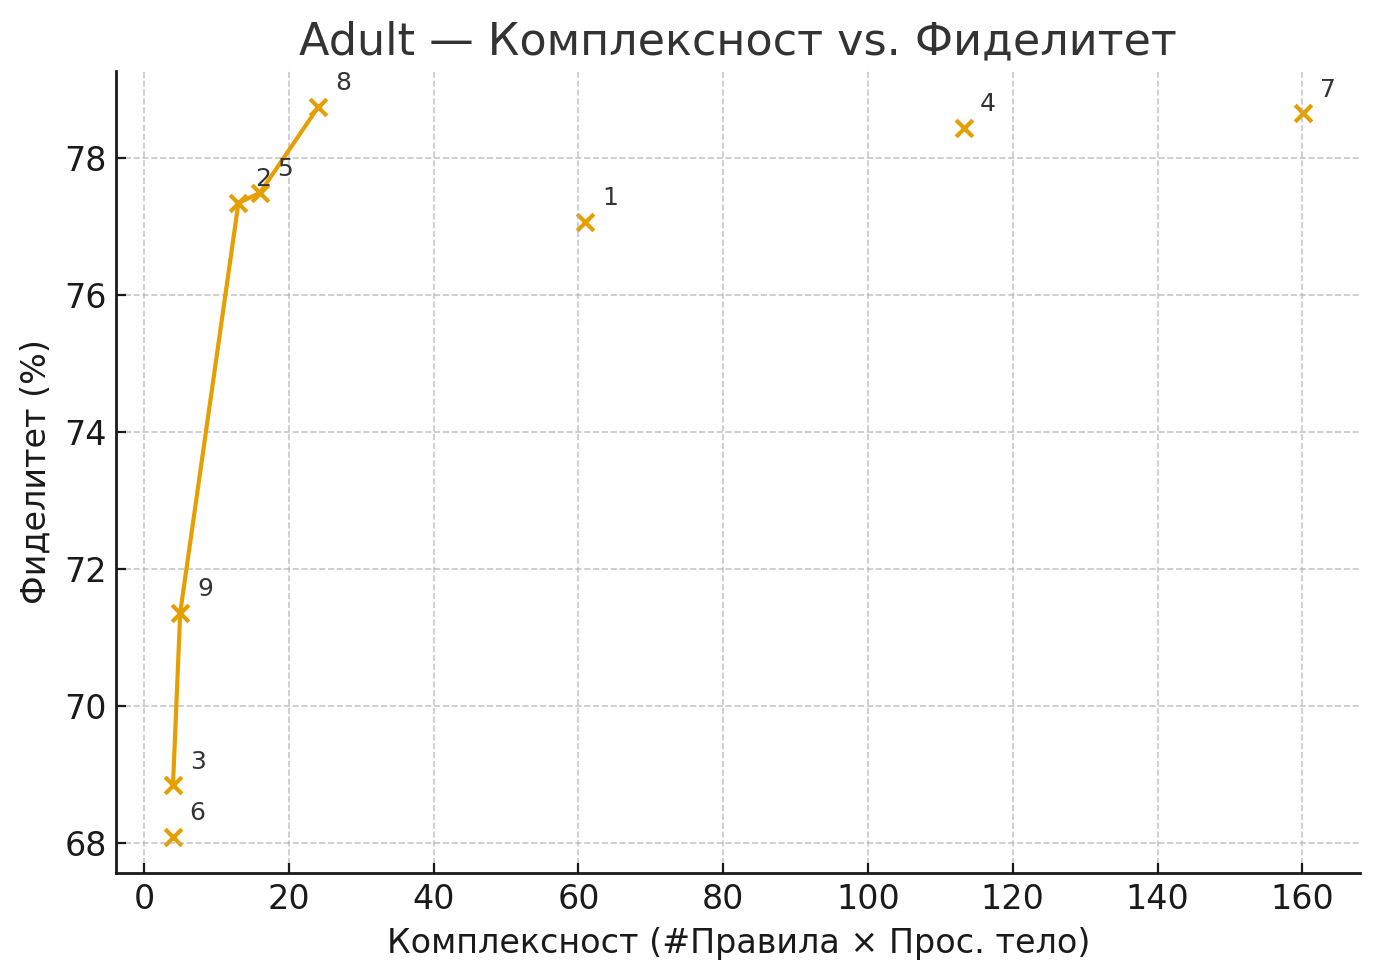
\includegraphics[width=.85\linewidth]{images/charts/adult-kompleksnost-fidelitet.png}
  \caption{Комплексност vs. Фиделитет — \textit{adult}.}
  \label{fig:adult-complexity-fidelity}
\end{figure}

Као и код фиделитета, већа комплексност донекле побољшава тачност, али добици после одређене тачке постају занемарљиви, Парето фронт помаже да се изабере модел који нуди најбољи однос тачности и једноставности, слично као код фиделитета, где све поставке сем \texttt{sweeper} дају резултате који имају тачност \textit{> 0.74}. Видети слику \ref{fig:adult-complexity-accuracy}.
\begin{figure}[H]
  \centering
  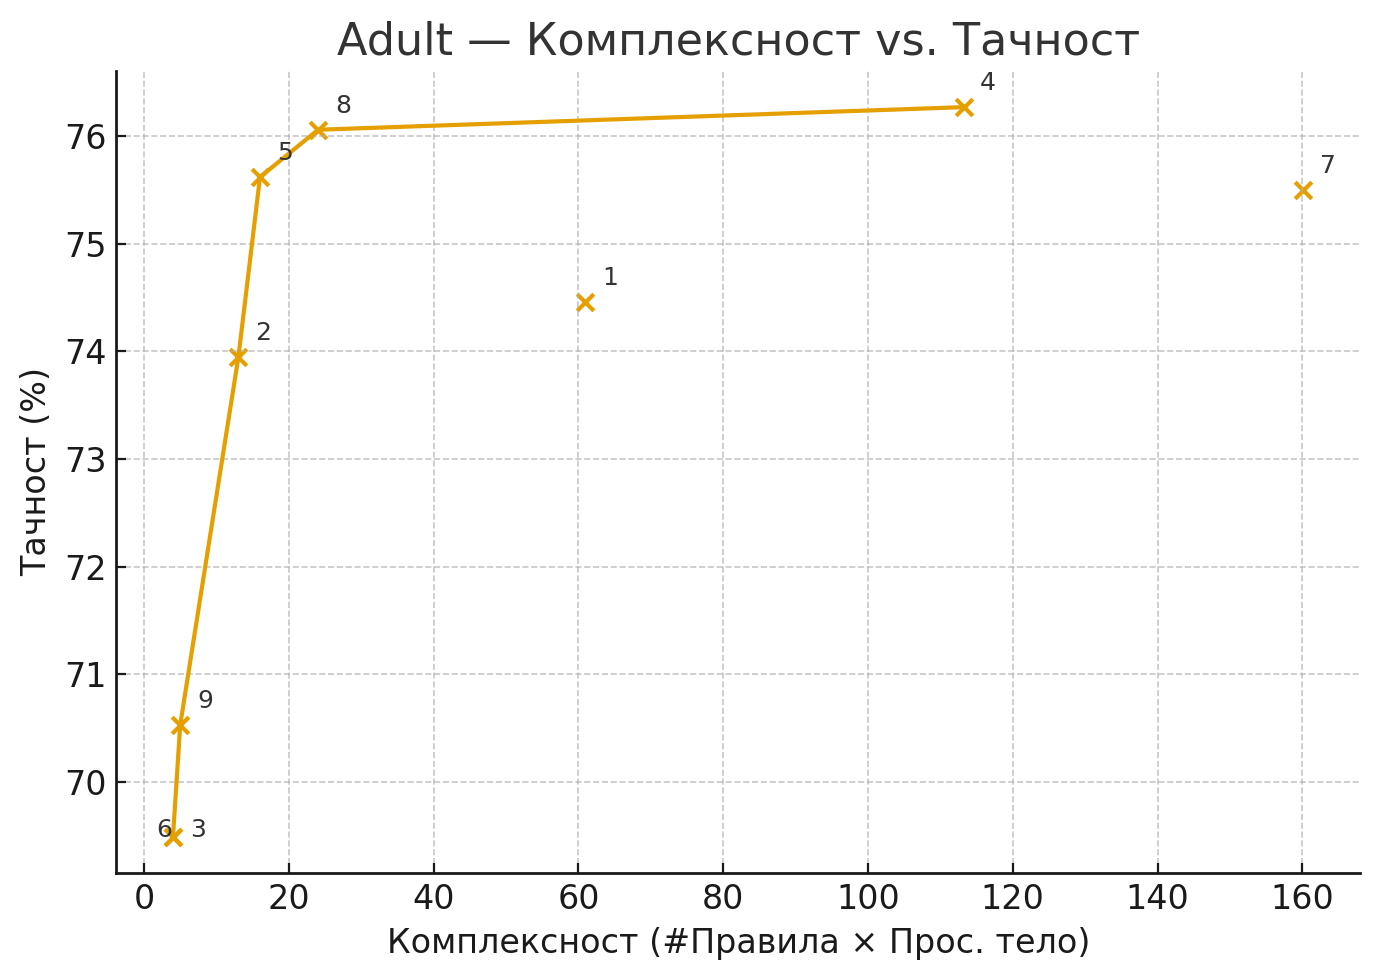
\includegraphics[width=.85\linewidth]{images/charts/adult-kompleksnost-tacnost.png}
  \caption{Комплексност vs. Тачност — \textit{adult}.}
  \label{fig:adult-complexity-accuracy}
\end{figure}

Постоји јасно опадање \textit{MCC} при преласку са \textit{sniper} на \textit{sweeper} поставке, што значи да смањивање комплексности доводи до губитка квалитета, а \textit{sniper} и \textit{sweet\_spot} дају најбољи резултат. Такође, \textit{DT} учитељ даје конзистентно најнижи \textit{MCC}, док \textit{RF} и \textit{XGB} дају сличне и боље резултате, што указује на предност ансамбл модела у овом случају. Видети слику \ref{fig:adult-mcc}.
\begin{figure}[H]
  \centering
  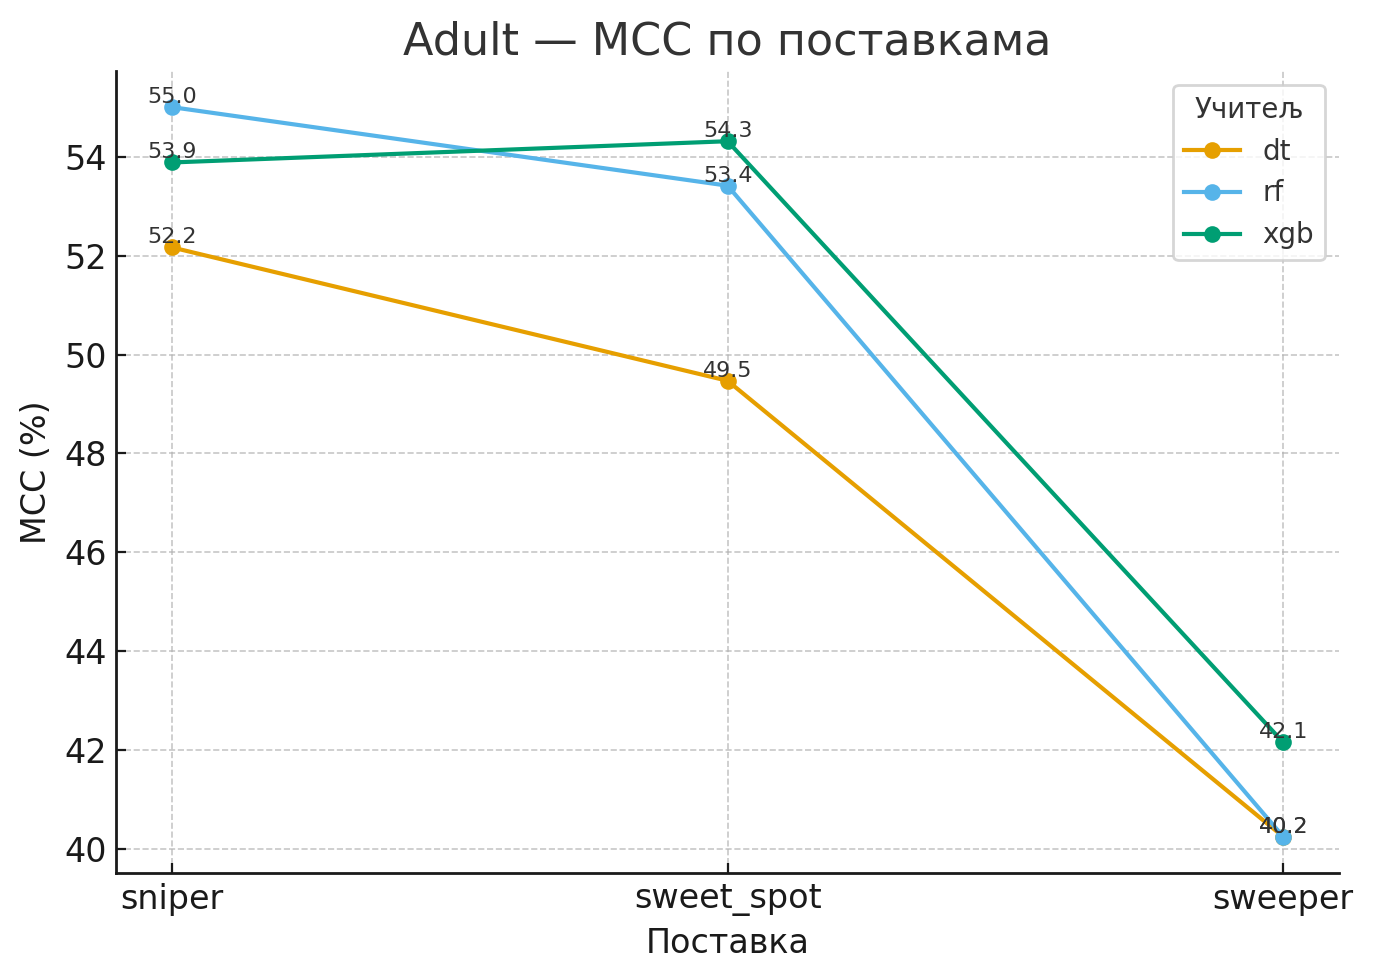
\includegraphics[width=.85\linewidth]{images/charts/adult-mcc.png}
  \caption{\textit{MCC} по поставкама — \textit{adult}.}
  \label{fig:adult-mcc}
\end{figure}

Табела \ref{tab:rules-top1-adult} приказује најбоље правило по комбинацији (датасет, учитељ, поставка). Правила су одабрана по највишој подршци.

\begin{table}[H]
\centering
\resizebox{\textwidth}{!}{
\begin{tabular}{@{}lllrrrrr@{}}
\toprule
\textbf{Скуп} & \textbf{Учитељ} & \textbf{Поставка} & \textbf{ИД правила} & \textbf{|Тело|} & \textbf{Подршка} & \textbf{Покривеност} & \textbf{Прецизност} \\
\midrule
adult    & dt  & sniper     & 19 & 3 & 174 & 0.0943 & 1.0000 \\
adult    & dt  & sweet\_spot& 3  & 1 & 196 & 0.1062 & 1.0000 \\
adult    & dt  & sweeper    & 2  & 1 & 196 & 0.1062 & 1.0000 \\
adult    & rf  & sniper     & 38 & 2 & 294 & 0.1565 & 1.0000 \\
adult    & rf  & sweet\_spot& 8  & 2 & 294 & 0.1565 & 1.0000 \\
adult    & rf  & sweeper    & 2  & 1 & 196 & 0.1033 & 0.9898 \\
adult    & xgb & sniper     & 52 & 3 & 220 & 0.1211 & 1.0000 \\
adult    & xgb & sweet\_spot& 11 & 2 & 294 & 0.1591 & 0.9830 \\
adult    & xgb & sweeper    & 2  & 1 & 196 & 0.1068 & 0.9898 \\
\bottomrule
\end{tabular}
}
\caption{Најбоље правило за скуп \textit{adult} по комбинацији (учитељ, поставка), бирано по највишој подршци.}
\label{tab:rules-top1-adult}
\end{table}

За скуп adult доминира нешто већа разноврсност издвојених правила. Једнолитерална клауза $capital\_gain=medium$ појављује се као најбоље у више учитеља и поставки, што указује на њену робусност као индикатора класе. Клауза $education=advanced\_degree \land marital\_status=married\_civ\_spouse$ доследно се јавља код \textit{RF} учитеља (\textit{sniper}, \textit{sweet\_spot}) и код \textit{XGB} учитеља (\textit{sweet\_spot}) са идентичном подршком, што потврђује њен значај за предвиђање високе зараде.

Поставке \textit{sniper} чешће фаворизују тролитералне клаузе мање покривености али веће специфичности (нпр. \textit{XGB}: $bachelors \land married \land hours>40$, \textit{DT}: $husband \land bachelors \land age\ 35–45$), док \textit{sweet\_spot} и \textit{sweeper} поставке преферирају једноставније клаузе шире примене, при чему прецизност зависи од самог атрибута, поједина једнолитерална правила као што је $capital\_gain = medium$ задржавају веома високу прецизност, док друга имају умерену.


Уочава се да више учитеља и поставки конзистентно издваја исте једно- или дволитералне клаузе, што указује на постојање стабилних и интерпретабилних правила, док комплексније клаузе омогућавају додавање специфичних услова који повећавају прецизност у ужим подскуповима података.

\paragraph{Напомена о наредним графиконима} У наредним графиконима, за сваку метрику, приказане су вредности у односу на учитеља и истину по свим комбинацијама учитељ/поставка. За сваку метрику приказан је засебан графикон.


На adult сету тачност према учитељу је у већини случајева виша од тачности према истини, што значи да дестилат чешће погађа учитељеве ознаке него што је заиста у праву, у \textit{sweeper} конфигурацијама се ово понекад преокреће, али доминира образац \emph{фиделитет > стварна тачност}. Претпоставка је да је учитељ увео одређену дозу шума у ознаке, коју дестилат довољно успешно имитира, али која смањује стварни квалитет. Видети слику \ref{fig:adult-acc}.
\begin{figure}[H]
  \centering
  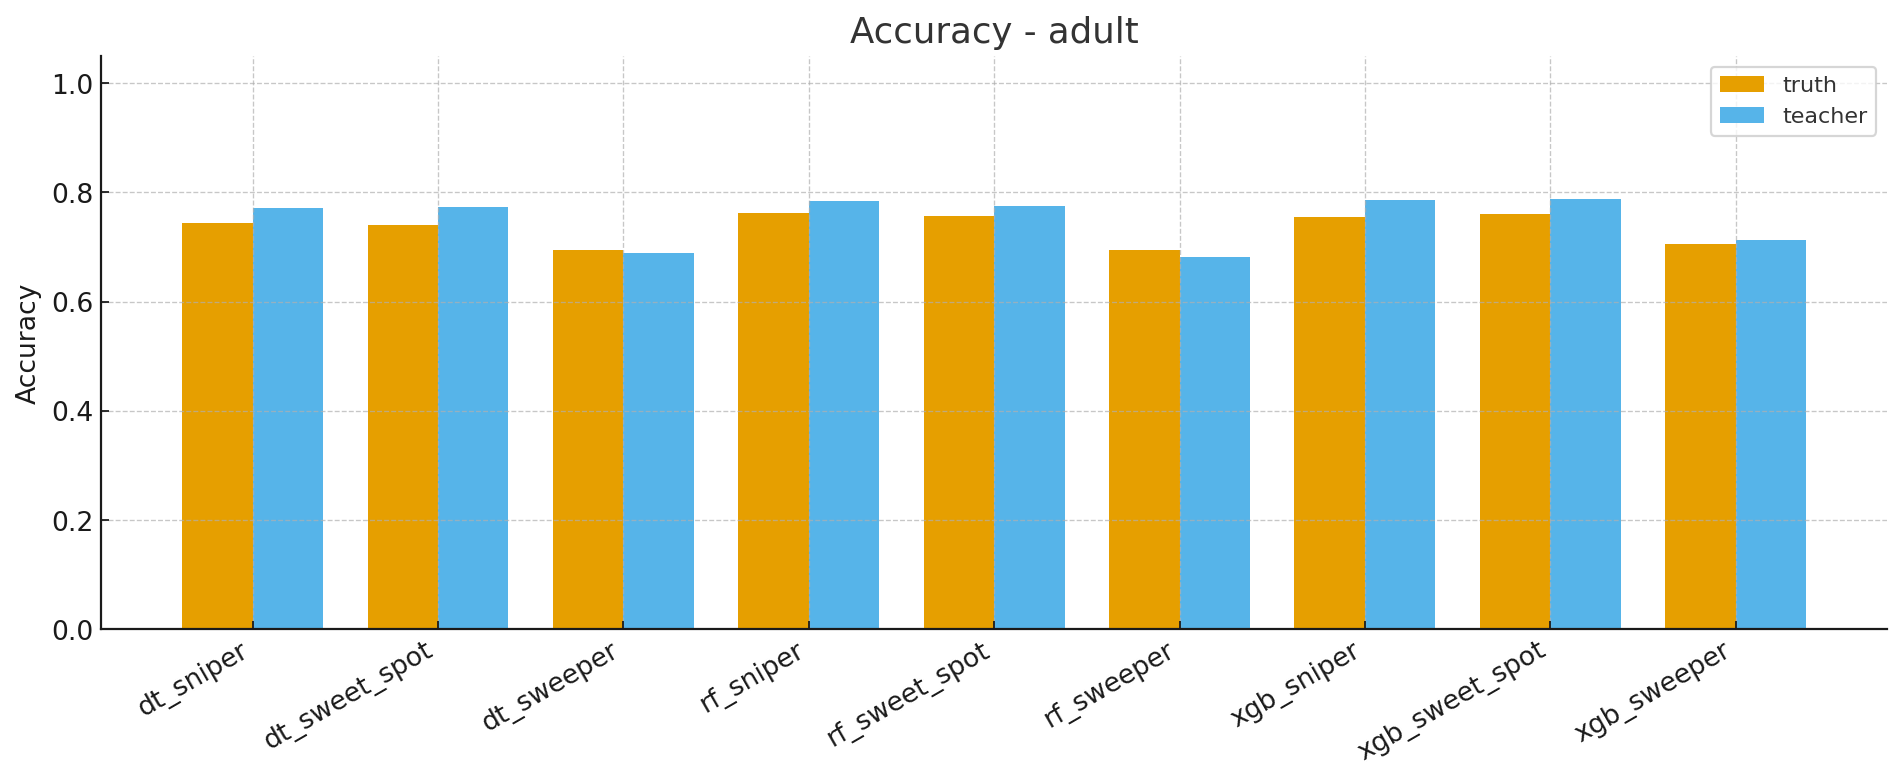
\includegraphics[width=.85\linewidth]{images/charts/accuracy_simple_adult.png}
  \caption{Accuracy — \textit{adult}.}
  \label{fig:adult-acc}
\end{figure}

Прецизност према учитељу је знатно виша од прецизности према истини у свим поставкама/моделима: када дестилат прогнозира „позитивно“, то се врло често поклапа са учитељем, али ређе са истинитим ознакама, висока верност позитивима учитеља, уз мању реалну прецизност. Опет, претпоставка је да учитељеве ознаке садрже шум који дестилат имитира, али генерализација није довољно добра. Видети слику \ref{fig:adult-acc}.
\begin{figure}[H]
  \centering
  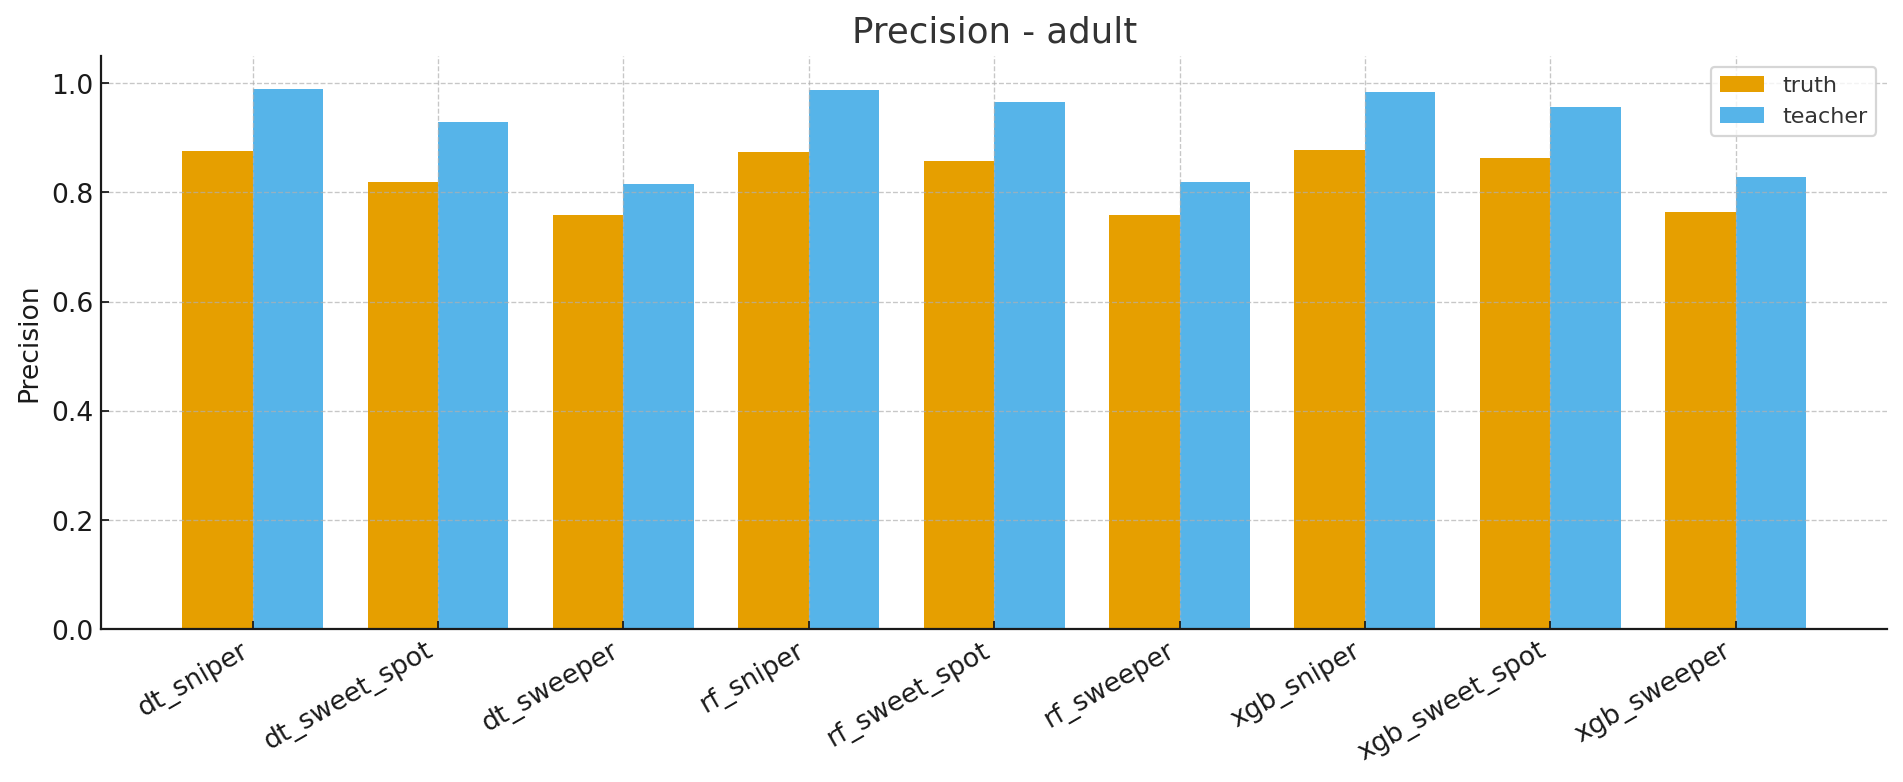
\includegraphics[width=.85\linewidth]{images/charts/precision_simple_adult.png}
  \caption{Precision — \textit{adult}.}
  \label{fig:adult-prec}
\end{figure}

Одзив према учитељу је у већини случајева мало већи или сличан одзиву према истини, што значи да дестилат боље „покрива“ учитељеве позитиве него стварне позитиве, у \textit{sweeper} поставкама одзив може пасти испод одзива према истини. Видети слику \ref{fig:adult-recall}.
\begin{figure}[H]
  \centering
  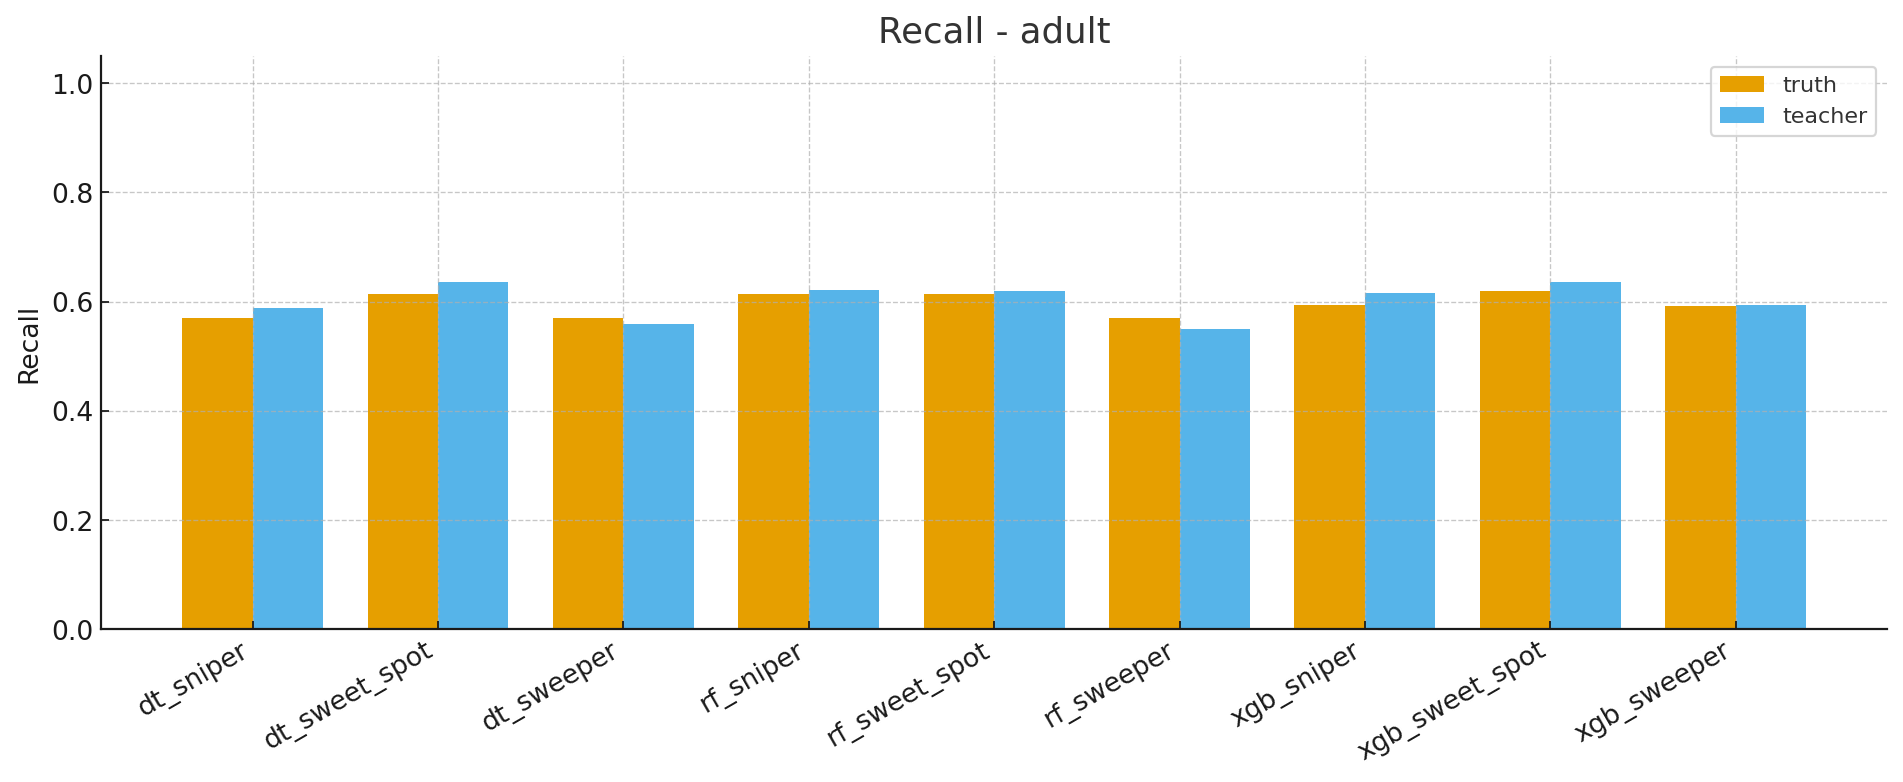
\includegraphics[width=.85\linewidth]{images/charts/recall_simple_adult.png}
  \caption{Recall — \textit{adult}.}
  \label{fig:adult-recall}
\end{figure}

F1 према учитељу је доследно изнад F1 према истини: баланс прецизности и одзива изгледа боље када се мери на учитељским ознакама него на истинитим, што указује на јаку имитацију понашања учитеља уз нешто слабији стварни квалитет. Видети слику \ref{fig:adult-f1}.
\begin{figure}[H]
  \centering
  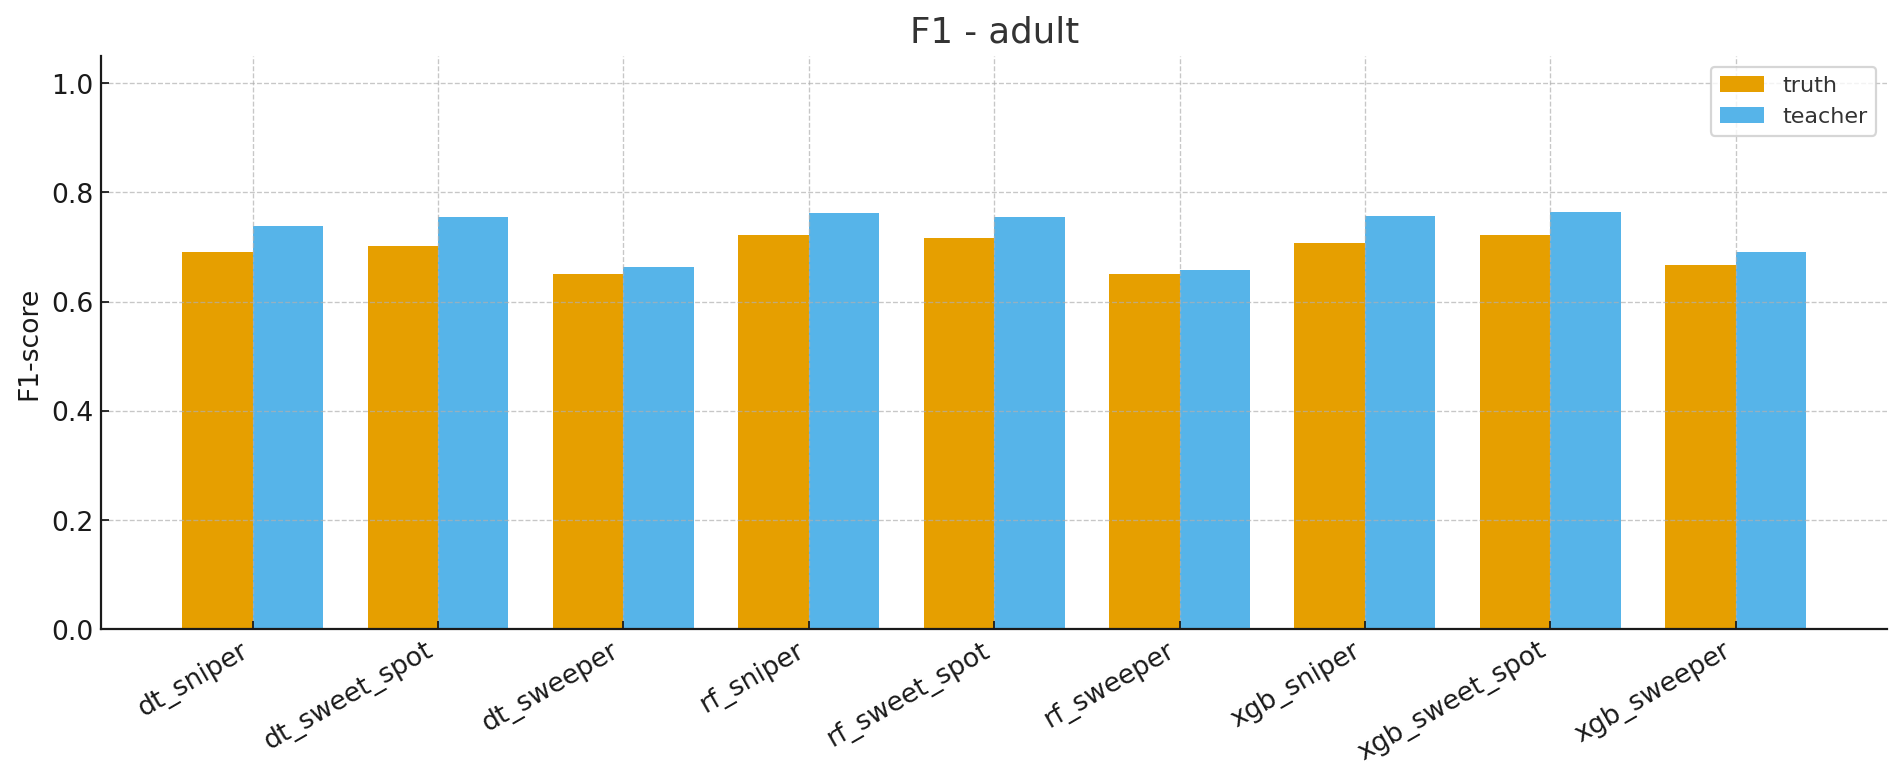
\includegraphics[width=.85\linewidth]{images/charts/f1_simple_adult.png}
  \caption{F1 — \textit{adult}.}
  \label{fig:adult-f1}
\end{figure}

\textit{MCC} према учитељу је у свим поставкама виши: укупни корелациони квалитет предвиђања дестилата боље се слаже са учитељем него са истином, што сугерише да су одлуке дестилата ближе учитељевој граници него стварној дистрибуцији ознака. Видети слику \ref{fig:adult-mcc-tt}.
\begin{figure}[H]
  \centering
  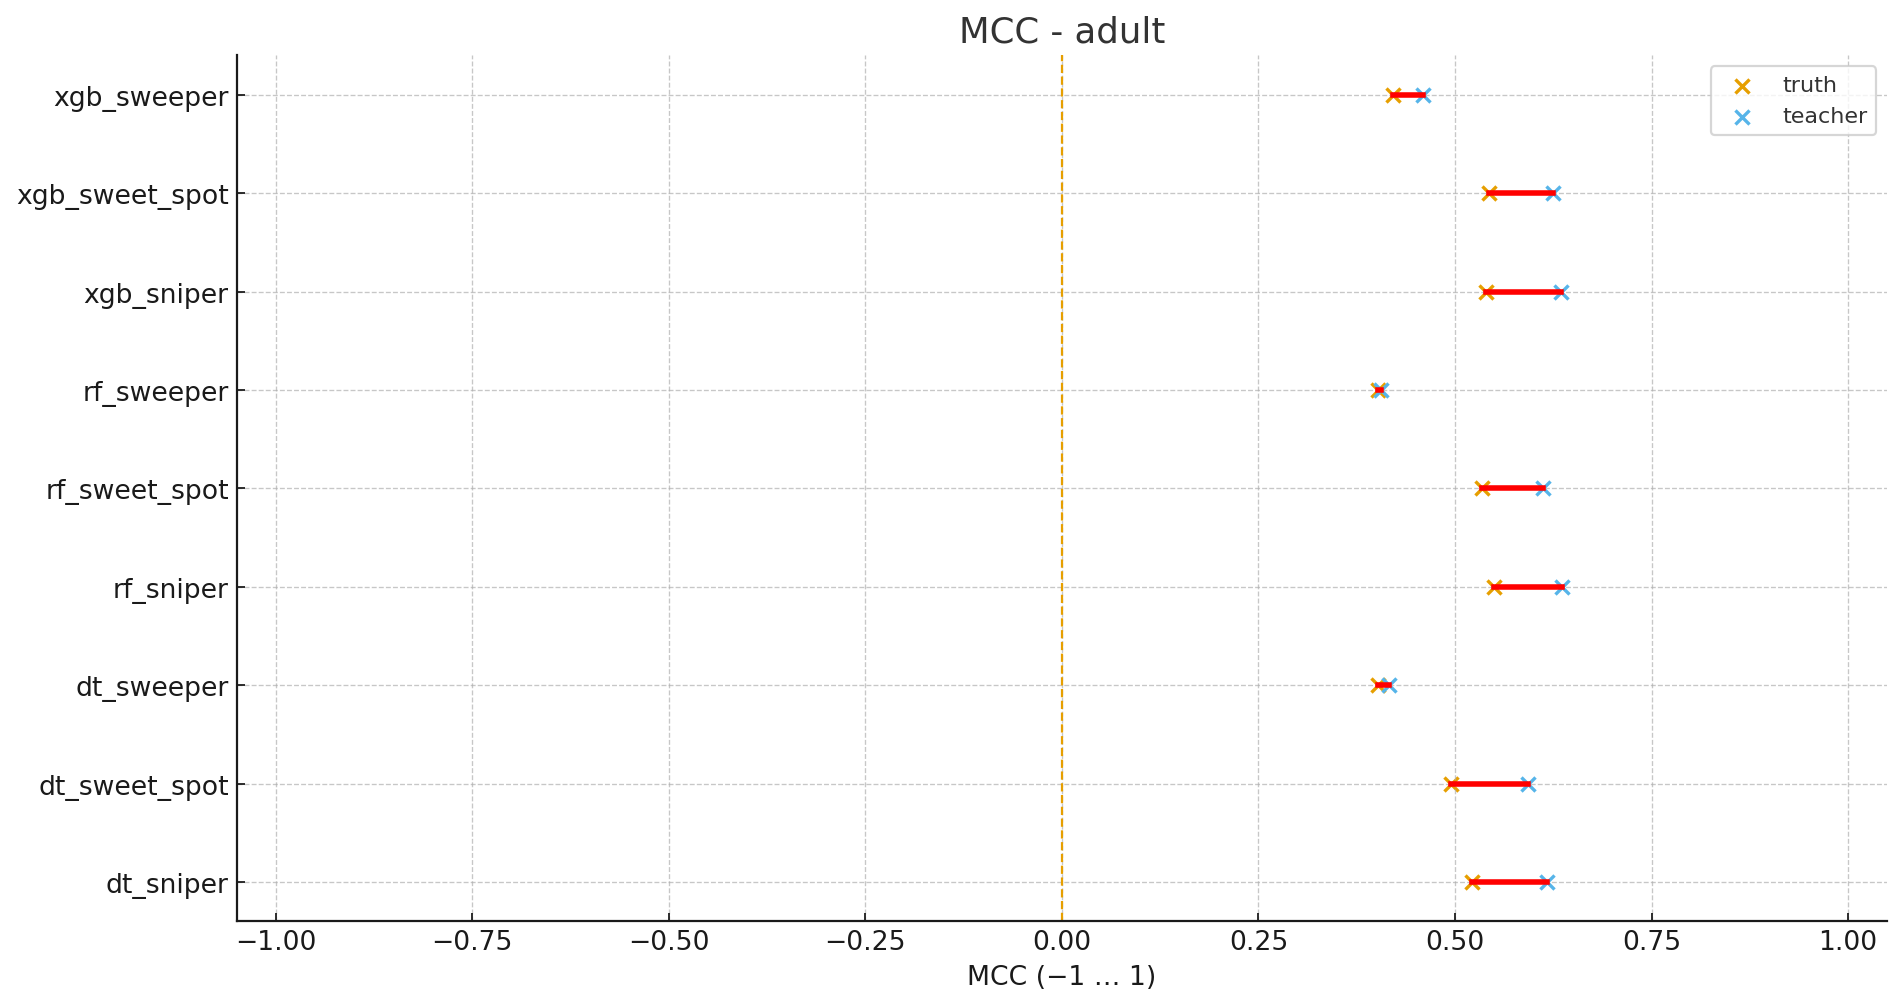
\includegraphics[width=.85\linewidth]{images/charts/mcc_simple_adult.png}
  \caption{\textit{MCC} — \textit{adult}.}
  \label{fig:adult-mcc-tt}
\end{figure}

\subsubsection*{Закључак — \textit{adult}}
Дестилација у Aleph-у открива уобичајени компромис између верности учитељу и стварне тачности према истини: фиделитет је редовно виши од тачности, што указује да дестилати веома успешно имитирају понашање учитеља, али не нужно побољшавају реалну генерализацију. Повећање сложености (више правила и дужа тела) доноси добитке који брзо опадају, \textit{sniper} и \textit{sweet\_spot} дају најбољи однос квалитета и интерпретабилности, док \textit{sweeper} пружа најједноставнија, али и слабија решења (нижи \textit{MCC}). У односу на учитеље, \textit{RF} и \textit{XGB} воде ка дестилатима са стабилнијим метрикама од \textit{DT}-а, што подржава избор ансамбла као учитеља кад је циљ висок фиделитет уз разумну сложеност.

Практично, за \textit{adult} је најисплативије дестилисати \textit{RF}/\textit{XGB} у \textit{sweet\_spot} режиму са умереним ограничењем дужине клаузе (3–4) и строжим \texttt{minacc} (≥0.7–0.8): добијају се компактни скуп(ови) правила који задржавају висок фиделитет и прихватљив реалан квалитет. Имајући у виду да су класе у оригиналу неуједначене (иако су у експерименту избалансиране \textit{undersampling}-ом), за продукциону примену препоручује се (i) провера калибрације и осетљивих метрика, (ii) анализа стабилности правила под различитим шемама дискритизације. Укратко: интерпретабилни дестилати на \textit{adult} могу верно да „преведу“ ансамбл учитеље у логичка правила уз минималан губитак перформанси, под условом да се пажљиво изабере зона компромиса између сложености и квалитета.

\subsection{Контрола компромиса прецизност-одзив}

У литератури је показано да се компромис прецизност-одзив у ИЛП-у може додатно контролисати ансамблирањем клауза по узору на \emph{Gleaner} \cite{Goadrich2006Gleaner}: кандидати се рангирају по одзиву на тренинг/валидацији, оса одзива се дели у $B$ биновa, у сваком бину задржава се до $K$ разноврсних клауза (нпр. по разликама у покривању), а одлука се формира правилом $L$-од-$K$ (пример је позитиван ако га покрива најмање $L$ клауза из датог бина). На тај начин се, без измене саме индукције, генерише читав скуп тачака на PR кривој и максимизује AURPC у окружењима са дисбалансом класа. Приступ је комплементаран „дестилатима“, који померају појединачне тачке кроз подешавања \texttt{evalfn}, \texttt{minacc} и \texttt{noise}. За евалуацију се препоручује угнежђена валидација хиперпараметара $(B,K,L)$ и bootstrap поређење AURPC у односу на базну поставку, уз контролу сложености дедупликацијом клауза, елиминацијом Pareto-доминираних кандидата у (recall, precision) простору и ограничавањем $K$ по бину. Поступак је тривијално паралелизабилан по биновима и/или по скуповима семена. 
